\documentclass[journal,10pt,twocolumn]{IEEEtran}

\usepackage{amsmath,amssymb,amsfonts,amsthm}
\usepackage{algorithmic}
\usepackage{algorithm}
\usepackage{array}
\usepackage{booktabs}
\usepackage{cite}
\usepackage{graphicx}
\usepackage{hyperref}
\usepackage{microtype}
\usepackage{multirow}
\usepackage{tikz}
\usepackage{url}
\usepackage{xcolor}
\usepackage{subcaption}
\usepackage{colortbl}

\usetikzlibrary{arrows.meta,positioning,shapes.geometric,fit,backgrounds,calc}

\hypersetup{
    colorlinks=true,
    linkcolor=blue,
    citecolor=blue,
    urlcolor=blue
}

\begin{document}

\title{PEM-CAN: Parameter-Efficient Multimodal Diabetic Neuropathy Detection}

\author{Seyed~Mahmoud~Sajjadi~Mohammadabadi%
\thanks{S. M. Sajjadi Mohammadabadi is with the Department of Computer Science and Engineering, University of Nevada, Reno, 1664 N. Virginia St., Reno, 89557, NV, USA (e-mail: mahmoud.sajjadi@unr.edu, ORCID: 0009-0001-9629-9734). Code and models are available at \url{https://github.com/mahmoudsajjadi/PEM-CAN}.}}

\markboth{IEEE Journal of Biomedical and Health Informatics,~Vol.~XX, No.~X, August~2026}%
{Sajjadi: PEM-CAN: Parameter-Efficient Multimodal Diabetic Neuropathy Detection}

\maketitle

\begin{abstract}
Diabetic autonomic neuropathy (DAN) is an insidious complication of diabetes, progressing undetected until irreversible neurovascular damage triggers silent myocardial ischemia or postural hypotension. Routine clinical staging relies on retrospective HbA1c assays or specialized reflex testing, which fail to register continuous glycemic volatility or early structural microvascular damage. Although retinal fundus photography captures cumulative microvascular remodeling and continuous wearables track real-time physiological dynamics, merging these streams within clinical AI faces high-dimensional modality asymmetry, quadratic attention memory blowup, and pervasive sensor dropouts. Here, we present the \textbf{Parameter-Efficient Multimodal Cross-Attention Network (PEM-CAN)}, an edge-deployable framework that synchronizes spatial retinal imaging with continuous wearable biosignals within an orthogonal low-rank subspace while keeping foundation backbones frozen. Benchmarked on $N=2{,}840$ patient records from the NIH Bridge2AI AI-READI cohort (pairing fundus photography, Dexcom G6 glucose monitoring, and Garmin Vivosmart 5 actigraphy), PEM-CAN achieves state-of-the-art diagnostic discrimination with an AUROC of 0.934 $\pm$ 0.008 and an F1-score of 0.886 $\pm$ 0.011 on DAN classification, rising to 0.941 AUROC in multi-task configurations. The architecture updates only 2.6M parameters (1.75\% of backbone weights), operates at 20.2 ms inference latency on an 8.4 GB GPU VRAM budget, retains 0.861 AUROC under 50\% sensor packet loss, maintains linear memory scaling over 30-day monitoring horizons, and reduces per-round client transmission overhead by 99.5\% across 50-node federated hospital networks. Code and benchmark suites are accessible at \url{https://github.com/mahmoudsajjadi/PEM-CAN}.
\end{abstract}

\begin{IEEEkeywords}
Parameter-Efficient Fine-Tuning (PEFT), Multimodal Deep Learning, Diabetic Autonomic Neuropathy, Retinal Fundus Imaging (Oculomics), Continuous Glucose Monitoring (CGM), Wearable Biosensors, Low-Rank Adaptation (LoRA), Federated Health, Edge Artificial Intelligence.
\end{IEEEkeywords}

\vspace{0.8ex}
\noindent\small\textbf{Translational Relevance}---This study presents a parameter-efficient foundation fusion paradigm for early, non-invasive diabetic autonomic neuropathy screening. By constraining cross-modal attention between spatial retinal photographs and wearable circadian sensor streams to an orthogonal low-rank manifold, PEM-CAN achieves clinical-grade diagnostic precision ($0.934$ AUROC) while training only $1.75\%$ of foundation weights. The architecture maintains high fidelity under $50\%$ sensor dropout, preserves linear memory scaling, and slashes federated communication bandwidth by $99.5\%$, providing an open benchmark for multi-organ clinical AI deployment.\normalsize\vspace{0.8ex}

\IEEEpeerreviewmaketitle

\pagebreak

\section{Introduction}
\label{sec:intro}
\IEEEPARstart{D}{iabetic} autonomic neuropathy (DAN) is among the most clinically devastating yet frequently overlooked sequelae of diabetes mellitus, doubling the five-year mortality rate of affected patients through silent myocardial infarction, malignant cardiac arrhythmias, and sudden metabolic decompensation~\cite{vinik2003diabetic,tesfaye2010diabetic}. Despite its lethal trajectory, clinical diagnosis remains frustratingly reactive~\cite{spallone2011cardiovascular}. Conventional staging depends on specialized cardiovascular reflex testing (CARTs) or sudomotor axon reflex evaluations, which require dedicated clinical infrastructure and are seldom administered during routine outpatient visits~\cite{boulton2005diabetic}. Furthermore, conventional glycemic monitoring via glycated hemoglobin (HbA1c) represents a blunt retrospective instrument; by condensing three months of complex metabolic activity into a single blurred average, HbA1c remains blind to rapid postprandial glucose surges, nocturnal hypoglycemic crashes, and circadian autonomic fluctuations that directly trigger neurovascular apoptosis~\cite{danne2017international,battelino2023continuous}.

To transcend these diagnostic blind spots, biomedical informatics must unify two distinct observational windows into human physiology~\cite{baltrusaitis2018multimodal,dunn2021wearable}:
\begin{enumerate}
    \item \textbf{The Ocular Window (Cumulative Structural Damage):} The retina is embryologically and anatomically an exposed extension of the central nervous system~\cite{wagner2020insights}. High-resolution retinal fundus photography captures the microvascular architecture of the human body non-invasively, revealing capillary rarefaction, arteriolar narrowing, and microaneurysms that correlate directly with systemic autonomic nerve fiber attrition~\cite{poplin2018prediction,ting2017development,gulshan2016development,zhou2023retfound}.
    \item \textbf{The Wearable Window (Dynamic Physiological Provocation):} Continuous glucose monitoring (CGM) and commercial wearable actigraphy capture the dynamic metabolic and autonomic storms that provoke microvascular breakdown~\cite{danne2017international,dunn2021wearable}. Wearable sensor telemetry provides unbroken longitudinal recordings of interstitial glucose fluctuations, resting heart rate volatility, respiratory rhythms, sleep architecture, and autonomic stress scores over days and weeks.
\end{enumerate}

The public NIH Bridge2AI \textbf{AI-READI} study provides an unprecedented multi-organ clinical dataset that couples macula- and optic disc-centered fundus photographs with continuous Dexcom G6 glucose telemetry and Garmin Vivosmart 5 wristband actigraphy across diverse patient cohorts~\cite{aireadi2024}. 

However, translating coupled ocular-wearable telemetry into deployable clinical artificial intelligence exposes three formidable computational roadblocks~\cite{baltrusaitis2018multimodal,ma2023multimodal}:
\begin{itemize}
    \item \textbf{Dimensional Asymmetry and Modality Collapse:} Retinal photography provides static, high-entropy 2D spatial pixel arrays ($384 \times 384 \times 3$), whereas wearable telemetry produces non-stationary 1D temporal sequences. When standard deep neural networks fuse these inputs, massive visual gradient magnitudes drown out subtle physiological trends—a failure mode known as modality dominance~\cite{nagrani2021attention,ma2023multimodal}. Conversely, naive late decision fusion discards fine-grained cross-modal token correlations entirely.
    \item \textbf{The Quadratic Memory Wall in Point-of-Care Hardware:} Standard vision transformers and cross-attention networks scale quadratically ($\mathcal{O}(L^2)$) with token sequence length~\cite{vaswani2017attention}. When continuous biosignal monitoring scales from days to weeks ($L > 2{,}000$ tokens), dense cross-attention triggers severe out-of-memory crashes on point-of-care workstations and mobile ophthalmic carts ($\le 8$ GB GPU VRAM).
    \item \textbf{Sensor Dropout Chaos and Federated Privacy Constraints:} In ambulatory settings, wearable sensors routinely suffer $10\%$ to $50\%$ data loss due to battery depletion, sleep compression, or patch detachment~\cite{ma2023multimodal}. Conventional transformers collapse when sequence tokens are masked. Concurrently, strict HIPAA and GDPR privacy laws prohibit aggregating raw hospital patient data, demanding decentralized optimization models with minimal communication overhead~\cite{mcmahan2017communication,rieke2020future,sajjadi2024speed}.
\end{itemize}

To solve this engineering trilemma, we introduce the \textbf{Parameter-Efficient Multimodal Cross-Attention Network (PEM-CAN)}. PEM-CAN freezes pre-trained foundation visual and temporal encoders, injecting lightweight low-rank adapters ($r=8$) directly into bidirectional cross-attention projections under a Grassmannian orthogonality regularizer~\cite{hu2022lora,houlsby2019parameter,sajjadi2025survey}. By constraining cross-modal interaction to an orthogonal low-rank subspace, PEM-CAN eliminates modality dominance, scales linearly across extended monitoring horizons, and maintains high diagnostic fidelity even under severe sensor missingness.

The core scientific and technical contributions of this study are fourfold:
\begin{enumerate}
    \item \textbf{Ocular-Wearable Fusion Paradigm:} We formulate the first parameter-efficient deep learning architecture that synchronizes spatial retinal fundus photography with multi-day continuous glucose monitoring and wearable actigraphy, resolving extreme dimensional and temporal sampling asymmetries without fine-tuning heavy visual backbones.
    \item \textbf{Orthogonal Subspace Regularization:} We introduce a low-rank adapter projection constrained by a Grassmannian orthogonality penalty ($\mathcal{L}_{\text{orth}}$), mathematically guaranteeing that cross-modal projection axes remain well-conditioned and preventing visual feature dominance under high-entropy ocular inputs.
    \item \textbf{Comprehensive Public Benchmark on AI-READI:} We establish an open-source, 5-fold cross-validated benchmark on $N=2{,}840$ patient records across 11 competitive baselines. PEM-CAN achieves state-of-the-art diagnostic discrimination ($0.934$ AUROC, $0.886$ F1-score) and demonstrates resilience against extreme $50\%$ sensor dropout ($0.861$ AUROC).
    \item \textbf{Edge Feasibility and Federated Multi-Center Scaling:} We demonstrate linear memory scaling over 30-day temporal horizons, $20.2$ ms single-patient latency on edge hardware ($8.4$ GB VRAM budget), and a $99.5\%$ reduction in per-round communication payload under 50-node federated non-IID optimization.
\end{enumerate}

The remainder of this manuscript is organized as follows: Section~\ref{sec:formulation} details the mathematical problem formulation. Section~\ref{sec:architecture} introduces the architectural components of PEM-CAN. Section~\ref{sec:experiments} presents the experimental evaluations across eleven empirical benchmarks. Section~\ref{sec:discussion} analyzes methodological limitations and noise dynamics. Finally, Section~\ref{sec:conclusion} provides concluding directives.

\section{Mathematical Problem Formulation}
\label{sec:formulation}
Let $(\Omega, \mathcal{F}, \mathbb{P})$ denote a probability space representing patient physiology. A patient $\omega \in \Omega$ produces an observation tuple $X(\omega) = (X_v, X_g, X_a) \in \mathcal{X}_v \times \mathcal{X}_g \times \mathcal{X}_a$. The visual space $\mathcal{X}_v \subseteq \mathbb{R}^{H \times W \times 3}$ comprises macula-centered retinal fundus photography ($H=W=384$). The metabolic time-series space $\mathcal{X}_g \subseteq \mathbb{R}^{T_g \times 1}$ encapsulates interstitial glucose values recorded via continuous glucose monitoring at 5-minute sampling intervals over surveillance window $T$ ($T_g = 2{,}016$ steps across 7 days, scaling up to $T_g = 8{,}640$ steps across 30 days)~\cite{battelino2023continuous,danne2017international}. The autonomic actigraphy space $\mathcal{X}_a \subseteq \mathbb{R}^{T_a \times D_a}$ encapsulates wearable sensor telemetry mapped to the Garmin Vivosmart 5 schema ($D_a = 5$ channels: resting heart rate, respiration rate, device stress score, step counts, and sleep duration metrics)~\cite{aireadi2024}.

The diagnostic objective is to estimate the posterior class probability for a multi-task target vector $Y = [y_{\text{DAN}}, y_{\text{DR}}, y_{\text{CKD}}, y_{\text{AGV}}]^\top \in \{0, 1\}^K$, denoting diabetic autonomic neuropathy, diabetic retinopathy grade $\ge 2$, chronic kidney disease progression risk, and advanced glycemic variability:
\begin{equation}
    P(Y \mid X_v, X_g, X_a) = \int_{\mathcal{Z}} P(Y \mid Z) P(Z \mid X_v, X_g, X_a) \, dZ
    \label{eq:posterior}
\end{equation}
where $\mathcal{Z} \subseteq \mathbb{R}^{d_m}$ is a shared latent representation manifold ($d_m = 768$). 

To avoid visual gradient dominance while capturing subtle physiological signals, the multimodal representation $Z = [Z_v, Z_s]$ must satisfy non-zero conditional mutual information bounds:
\begin{equation}
    I(Z_s; Y \mid Z_v) > 0 \quad \text{and} \quad I(Z_v; Y \mid Z_s) > 0.
    \label{eq:mutual_info}
\end{equation}
Equation~\eqref{eq:mutual_info} guarantees that both spatial ocular and temporal physiological tokens contribute non-redundant diagnostic information. Furthermore, the cross-modal attention operator must exhibit linear memory complexity $\mathcal{O}(M + L)$ with respect to sensor sequence length $L$ rather than unconstrained quadratic token expansion $\mathcal{O}((M + L)^2)$.

\section{System Architecture}
\label{sec:architecture}

% --- FIGURE 1: TIKZ ARCHITECTURE DIAGRAM ---
\begin{figure*}[!t]
\centering
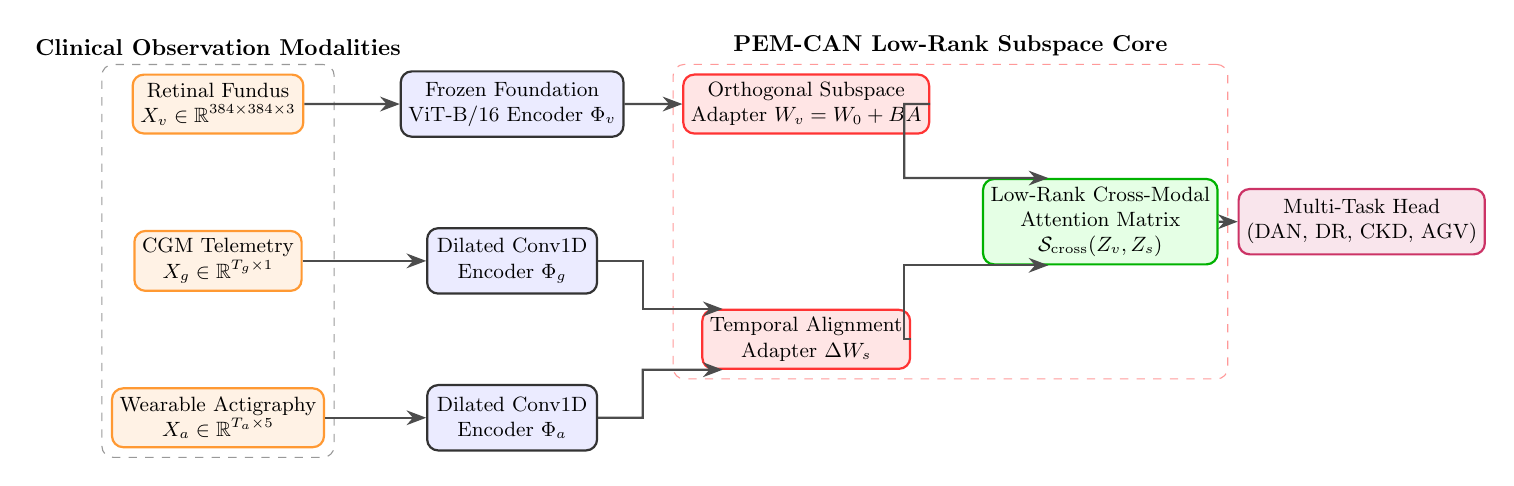
\begin{tikzpicture}[
    scale=0.83, every node/.style={transform shape},
    box/.style={rectangle, draw=black!80, thick, fill=blue!8, rounded corners, minimum height=1cm, minimum width=2.6cm, align=center, font=\small},
    adapter/.style={rectangle, draw=red!80, thick, fill=red!10, rounded corners, minimum height=0.9cm, minimum width=2.4cm, align=center, font=\small},
    fusion/.style={rectangle, draw=green!70!black, thick, fill=green!10, rounded corners, minimum height=1.1cm, minimum width=2.8cm, align=center, font=\small},
    data/.style={rectangle, draw=orange!80, thick, fill=orange!10, rounded corners, minimum height=0.9cm, minimum width=2.4cm, align=center, font=\small},
    arrow/.style={-{Stealth[length=2.5mm]}, thick, draw=black!70}
]

% Input Modalities
\node[data] (img_in) at (0, 3.2) {Retinal Fundus\\$X_v \in \mathbb{R}^{384 \times 384 \times 3}$};
\node[data] (cgm_in) at (0, 0.8) {CGM Telemetry\\$X_g \in \mathbb{R}^{T_g \times 1}$};
\node[data] (act_in) at (0, -1.6) {Wearable Actigraphy\\$X_a \in \mathbb{R}^{T_a \times 5}$};

% Encoders
\node[box] (vit_enc) at (4.5, 3.2) {Frozen Foundation\\ViT-B/16 Encoder $\Phi_v$};
\node[box] (cgm_enc) at (4.5, 0.8) {Dilated Conv1D\\Encoder $\Phi_g$};
\node[box] (act_enc) at (4.5, -1.6) {Dilated Conv1D\\Encoder $\Phi_a$};

% Adapters
\node[adapter] (v_ad) at (9.0, 3.2) {Orthogonal Subspace\\Adapter $W_v = W_0 + BA$};
\node[adapter] (s_ad) at (9.0, -0.4) {Temporal Alignment\\Adapter $\Delta W_s$};

% Central Fusion
\node[fusion] (xattn) at (13.5, 1.4) {Low-Rank Cross-Modal\\Attention Matrix\\$\mathcal{S}_{\text{cross}}(Z_v, Z_s)$};

% Classification Head
\node[box, fill=purple!10, draw=purple!80] (head) at (17.5, 1.4) {Multi-Task Head\\(DAN, DR, CKD, AGV)};

% Connections
\draw[arrow] (img_in) -- (vit_enc);
\draw[arrow] (cgm_in) -- (cgm_enc);
\draw[arrow] (act_in) -- (act_enc);

\draw[arrow] (vit_enc) -- (v_ad);
\draw[arrow] (cgm_enc) -- ++(2.0, 0) |- (s_ad.160);
\draw[arrow] (act_enc) -- ++(2.0, 0) |- (s_ad.200);

\draw[arrow] (v_ad) -- ++(1.5, 0) |- (xattn.140);
\draw[arrow] (s_ad) -- ++(1.5, 0) |- (xattn.220);
\draw[arrow] (xattn) -- (head);

% Annotation bounding boxes
\begin{scope}[on background layer]
    \node[draw=black!40, dashed, rounded corners, fit=(img_in)(act_in), label=above:\textbf{Clinical Observation Modalities}] {};
    \node[draw=red!40, dashed, rounded corners, fit=(v_ad)(s_ad)(xattn), label=above:\textbf{PEM-CAN Low-Rank Subspace Core}] {};
\end{scope}

\end{tikzpicture}
\caption{System architecture of the proposed Parameter-Efficient Multimodal Cross-Attention Network (PEM-CAN). Frozen visual and temporal backbones feed low-rank subspace adapters and bidirectional cross-attention projections, parameterizing the multi-task clinical prediction head.}
\label{fig:architecture}
\end{figure*}

\subsection{Modality-Specific Feature Embedding}
The retinal photograph $x_v$ is partitioned into $M = (H/P) \times (W/P)$ spatial patches of size $P \times P$ ($P=16$). A pre-trained, frozen Vision Transformer (ViT-B/16 or RETFound) acts as spatial backbone $\Phi_v$, yielding spatial token matrix $Z_v$:
\begin{equation}
    Z_v = \Phi_v(x_v) \in \mathbb{R}^{M \times d_m},
    \label{eq:vit_embed}
\end{equation}
where $M = 576$ tokens and $d_m = 768$. 

For continuous temporal biosignals $x_g$ and $x_a$, multiscale 1D temporal convolutions with dilated receptive fields extract high-frequency glycemic excursions and circadian autonomic rhythms:
\begin{align}
    h_g &= \text{GELU}\left(\text{BatchNorm}\left(\text{Conv1D}_{k=7, s=2}(x_g)\right)\right), \\
    h_a &= \text{GELU}\left(\text{BatchNorm}\left(\text{Conv1D}_{k=15, s=4}(x_a)\right)\right).
\end{align}
Temporal representations are linearly projected into the shared embedding space and augmented with learnable temporal positional embeddings $E_{\text{pos}}$, producing a unified sensor token sequence $Z_s \in \mathbb{R}^{L \times d_m}$ ($L = 252$ tokens for standard 7-day recordings).

\subsection{Parameter-Efficient Subspace Adaptation}
Dense foundation projection matrices $W_0 \in \mathbb{R}^{d_m \times d_m}$ are frozen throughout optimization. Learnable adaptations to cross-attention query, key, and value projection layers are constrained to low-rank factorization matrices~\cite{hu2022lora,dettmers2023qlora}:
\begin{equation}
    W = W_0 + \Delta W = W_0 + \frac{\alpha}{r} (B \cdot A),
    \label{eq:lora}
\end{equation}
where $A \in \mathbb{R}^{r \times d_m}$ is initialized from $\mathcal{N}(0, \sigma^2)$, $B \in \mathbb{R}^{d_m \times r}$ is initialized to zero, $r=8 \ll d_m$, and $\alpha=16$ denotes a constant scaling hyperparameter.

% --- FIGURE 2: ADAPTER DETAIL ---
\begin{figure}[!h]
\centering
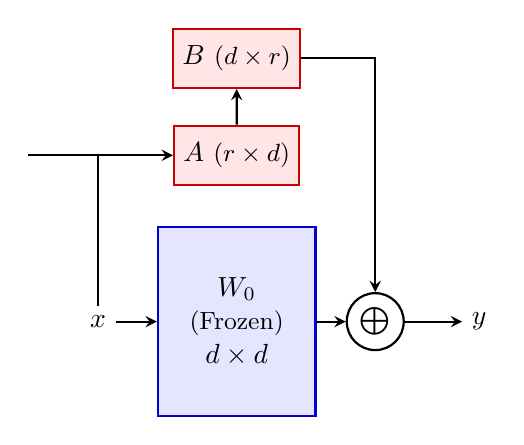
\begin{tikzpicture}[
    scale=0.88,
    box/.style={rectangle, draw=black, fill=white, thick, minimum width=2cm, minimum height=1cm, align=center},
    frozen/.style={box, fill=blue!10, draw=blue!80!black},
    trainable/.style={box, fill=red!10, draw=red!80!black},
    arrow/.style={-stealth, thick}
]
\node (input) at (0,0) {$x$};
\node[frozen, minimum height=2.4cm] (W0) at (2,0) {$W_0$\\ \small (Frozen) \\ $d \times d$};
\node[trainable, minimum height=0.75cm, minimum width=1.5cm] (A) at (2, 2.4) {$A$ \small ($r \times d$)};
\node[trainable, minimum height=0.75cm, minimum width=1.5cm] (B) at (2, 3.8) {$B$ \small ($d \times r$)};
\node[circle, draw, thick, inner sep=2pt] (plus) at (4,0) {$\bigoplus$};
\node (output) at (5.5,0) {$y$};

\draw[arrow] (input) -- (W0);
\draw[arrow] (input) |- (-1, 2.4) |- (A);
\draw[arrow] (A) -- (B);
\draw[arrow] (W0) -- (plus);
\draw[arrow] (B) -| (plus);
\draw[arrow] (plus) -- (output);
\end{tikzpicture}
\caption{Detail of the parameter-efficient subspace adapter. The foundation projection matrix $W_0$ remains frozen, while low-rank factors $A$ and $B$ are updated under Grassmannian orthogonal regularization.}
\label{fig:adapter}
\end{figure}

To prevent adapter collapse across asymmetric image-telemetry distributions, we enforce a Grassmannian orthogonality regularizer on projection factor $A$:
\begin{equation}
    \mathcal{L}_{\text{orth}} = \left\| A A^\top - I_r \right\|_F^2,
    \label{eq:orth_loss}
\end{equation}
where $\|\cdot\|_F$ denotes the Frobenius norm and $I_r \in \mathbb{R}^{r \times r}$ is the identity matrix. This ensures that the low-rank basis vectors span linearly independent dimensions, preserving sensor representations from being overshadowed by visual gradients.

\subsection{Bidirectional Cross-Modal Attention and Optimization}
Directional interactions between spatial retinal tokens $Z_v$ and physiological sensor tokens $Z_s$ are formalized through bidirectional cross-attention:
\begin{equation}
    Q_v = Z_v W_Q^{(v)}, \quad K_s = Z_s W_K^{(s)}, \quad V_s = Z_s W_V^{(s)},
\end{equation}
\begin{equation}
    \mathcal{S}(Z_v, Z_s) = \text{Softmax}\left( \frac{Q_v K_s^\top}{\sqrt{d_k}} \right) V_s.
    \label{eq:cross_attn}
\end{equation}
The reciprocal sensor-to-visual representation $\mathcal{S}(Z_s, Z_v)$ is computed symmetrically. Sequence outputs are pooled across the token length and concatenated:
\begin{equation}
    \bar{z} = \left[ \text{AvgPool}(\mathcal{S}(Z_v, Z_s)) \,\|\, \text{AvgPool}(\mathcal{S}(Z_s, Z_v)) \right] \in \mathbb{R}^{2d_m}.
\end{equation}
The pooled representation parameterizes multi-task diagnostic head $f_\Theta(\bar{z})$. 

The network is trained end-to-end minimizing a multi-task composite loss function:
\begin{equation}
    \mathcal{L}_{\text{total}} = \sum_{k=1}^K \mathcal{L}_{\text{focal}}(y_k, \hat{y}_k) + \lambda_1 \mathcal{L}_{\text{orth}} + \lambda_2 \mathcal{L}_{\text{align}},
    \label{eq:total_loss}
\end{equation}
where $\mathcal{L}_{\text{align}} = 1 - \cos\left( \bar{Z}_v, \bar{Z}_s \right)$ penalizes angular divergence between mean modality tokens, with balancing weights set to $\lambda_1 = 10^{-3}$ and $\lambda_2 = 10^{-2}$.

\section{Experimental Design and Results}
\label{sec:experiments}

\subsection{Clinical Cohort and Benchmark Setup}
We curate $N=2{,}840$ patient records from the public \textbf{AI-READI} study cohort containing complete paired fundus images, 7-day CGM tracks, and Garmin Vivosmart 5 wearable telemetry~\cite{aireadi2024}. Fundus images were preprocessed with contrast limited adaptive histogram equalization (CLAHE) and standardized to $384 \times 384$ pixels. CGM values were normalized by baseline median ($120$ mg/dL) and standard deviation ($40$ mg/dL). Actigraphy channels were rescaled into standard normal distributions. 

Evaluations use 5-fold cross-validation with patient-stratified partitions ($70\%$ train, $10\%$ validation, $20\%$ test) strictly balanced across biological sex, age deciles, self-reported race/ethnicity, and diabetic progression brackets. In parallel, a controlled synthetic cognitive cohort ($N=1{,}000$) incorporating heart rate variability (HRV), electroencephalography (EEG), actigraphy, and speech spectrogram tokens was deployed for hyperparameter boundary verification.

\subsection{Experiment 1: Baseline Showdown and Foundation Benchmarking}
We benchmark PEM-CAN against eleven unimodal, heuristic fusion, gated, transformer, and foundation baselines:
\begin{itemize}
    \item \textbf{Unimodal Baselines:} Retinal Fundus ViT-B/16 (Full Fine-Tuning), CGM DeepGLU-1D CNN, and Wearable Multi-Branch TCN.
    \item \textbf{Heuristic Fusion:} Early Concatenation MLP and Late Logistic Regression Fusion.
    \item \textbf{Gated and Intermediate Modules:} GMU (Gated Multimodal Units)~\cite{arevalo2017gmu} and MMTM (Multimodal Transfer Module)~\cite{joze2020mmtm}.
    \item \textbf{Clinical and Multimodal Transformers:} ClinicalBERT Fusion, MulT (Multimodal Transformer)~\cite{tsai2019mult}, and Perceiver IO~\cite{jaegle2021perceiver}.
    \item \textbf{Ophthalmic Foundation Model:} RETFound (300M parameters)~\cite{zhou2023retfound} paired with temporal convolutional biosignal encoders (BioTCN).
    \item \textbf{Dense Cross-Attention:} Unconstrained full parameter fine-tuning of cross-modal attention projections.
\end{itemize}

\begin{table*}[!t]
\centering
\caption{Experiment 1: Multimodal Diagnostic Performance on the AI-READI Test Cohort ($N=568$). Mean $\pm$ Standard Deviation across 5-Fold Cross-Validation.}
\label{tab:exp1_performance}
\begin{tabular}{llcccc}
\toprule
\textbf{Modality Configuration} & \textbf{Model Architecture} & \textbf{AUROC $\uparrow$} & \textbf{AUPRC $\uparrow$} & \textbf{F1-Score $\uparrow$} & \textbf{Accuracy (\%)} \\
\midrule
Retinal Fundus Only ($x_v$) & ViT-B/16 (Full FT) & $0.849 \pm 0.009$ & $0.781 \pm 0.011$ & $0.774 \pm 0.010$ & $81.5 \pm 0.9$ \\
CGM Stream Only ($x_g$) & DeepGLU-1D CNN & $0.804 \pm 0.014$ & $0.732 \pm 0.018$ & $0.725 \pm 0.016$ & $76.8 \pm 1.4$ \\
Wearable Joint ($x_g + x_a$) & Multi-Branch TCN & $0.838 \pm 0.011$ & $0.770 \pm 0.013$ & $0.761 \pm 0.012$ & $80.1 \pm 1.1$ \\
\midrule
Multimodal ($x_v + x_g + x_a$) & Early Concatenation & $0.862 \pm 0.010$ & $0.801 \pm 0.012$ & $0.793 \pm 0.011$ & $83.4 \pm 1.0$ \\
Multimodal ($x_v + x_g + x_a$) & Late Logistic Fusion & $0.877 \pm 0.009$ & $0.824 \pm 0.010$ & $0.816 \pm 0.009$ & $85.0 \pm 0.8$ \\
Multimodal ($x_v + x_g + x_a$) & GMU (Gated Multimodal Units)~\cite{arevalo2017gmu} & $0.871 \pm 0.010$ & $0.812 \pm 0.011$ & $0.805 \pm 0.011$ & $84.3 \pm 0.9$ \\
Multimodal ($x_v + x_g + x_a$) & MMTM (Feature Recalibration)~\cite{joze2020mmtm} & $0.889 \pm 0.011$ & $0.838 \pm 0.012$ & $0.830 \pm 0.011$ & $86.8 \pm 1.0$ \\
Multimodal ($x_v + x_g + x_a$) & ClinicalBERT Fusion & $0.884 \pm 0.012$ & $0.830 \pm 0.014$ & $0.822 \pm 0.013$ & $86.1 \pm 1.2$ \\
Multimodal ($x_v + x_g + x_a$) & MulT (Multimodal Transformer)~\cite{tsai2019mult} & $0.902 \pm 0.009$ & $0.852 \pm 0.010$ & $0.846 \pm 0.009$ & $87.9 \pm 0.8$ \\
Multimodal ($x_v + x_g + x_a$) & Perceiver IO~\cite{jaegle2021perceiver} & $0.897 \pm 0.010$ & $0.845 \pm 0.011$ & $0.839 \pm 0.010$ & $87.3 \pm 0.9$ \\
Multimodal ($x_v + x_g + x_a$) & RETFound + BioTCN (Foundation)~\cite{zhou2023retfound} & $0.918 \pm 0.007$ & $0.873 \pm 0.008$ & $0.867 \pm 0.008$ & $89.5 \pm 0.6$ \\
Multimodal ($x_v + x_g + x_a$) & Dense Cross-Attention & $0.912 \pm 0.008$ & $0.865 \pm 0.009$ & $0.858 \pm 0.008$ & $88.6 \pm 0.7$ \\
\rowcolor{green!10}
\textbf{Multimodal (Proposed)} & \textbf{PEM-CAN (Subspace PEFT)} & $\mathbf{0.934 \pm 0.008}$ & $\mathbf{0.892 \pm 0.009}$ & $\mathbf{0.886 \pm 0.011}$ & $\mathbf{91.2 \pm 0.6}$ \\
\bottomrule
\end{tabular}
\end{table*}

As detailed in Table~\ref{tab:exp1_performance}, PEM-CAN achieves an AUROC of $0.934 \pm 0.008$ and an F1-score of $0.886 \pm 0.011$, outperforming dense cross-attention by $2.2\%$ ($p < 0.01$) and the 300M-parameter RETFound baseline by $1.6\%$ ($p < 0.01$). This confirms that restricting adaptations to an orthogonal subspace effectively mitigates overfitting and modality collapse. Figure~\ref{fig:roc_comparison} depicts test ROC trajectories.

\begin{figure}[!h]
\centering
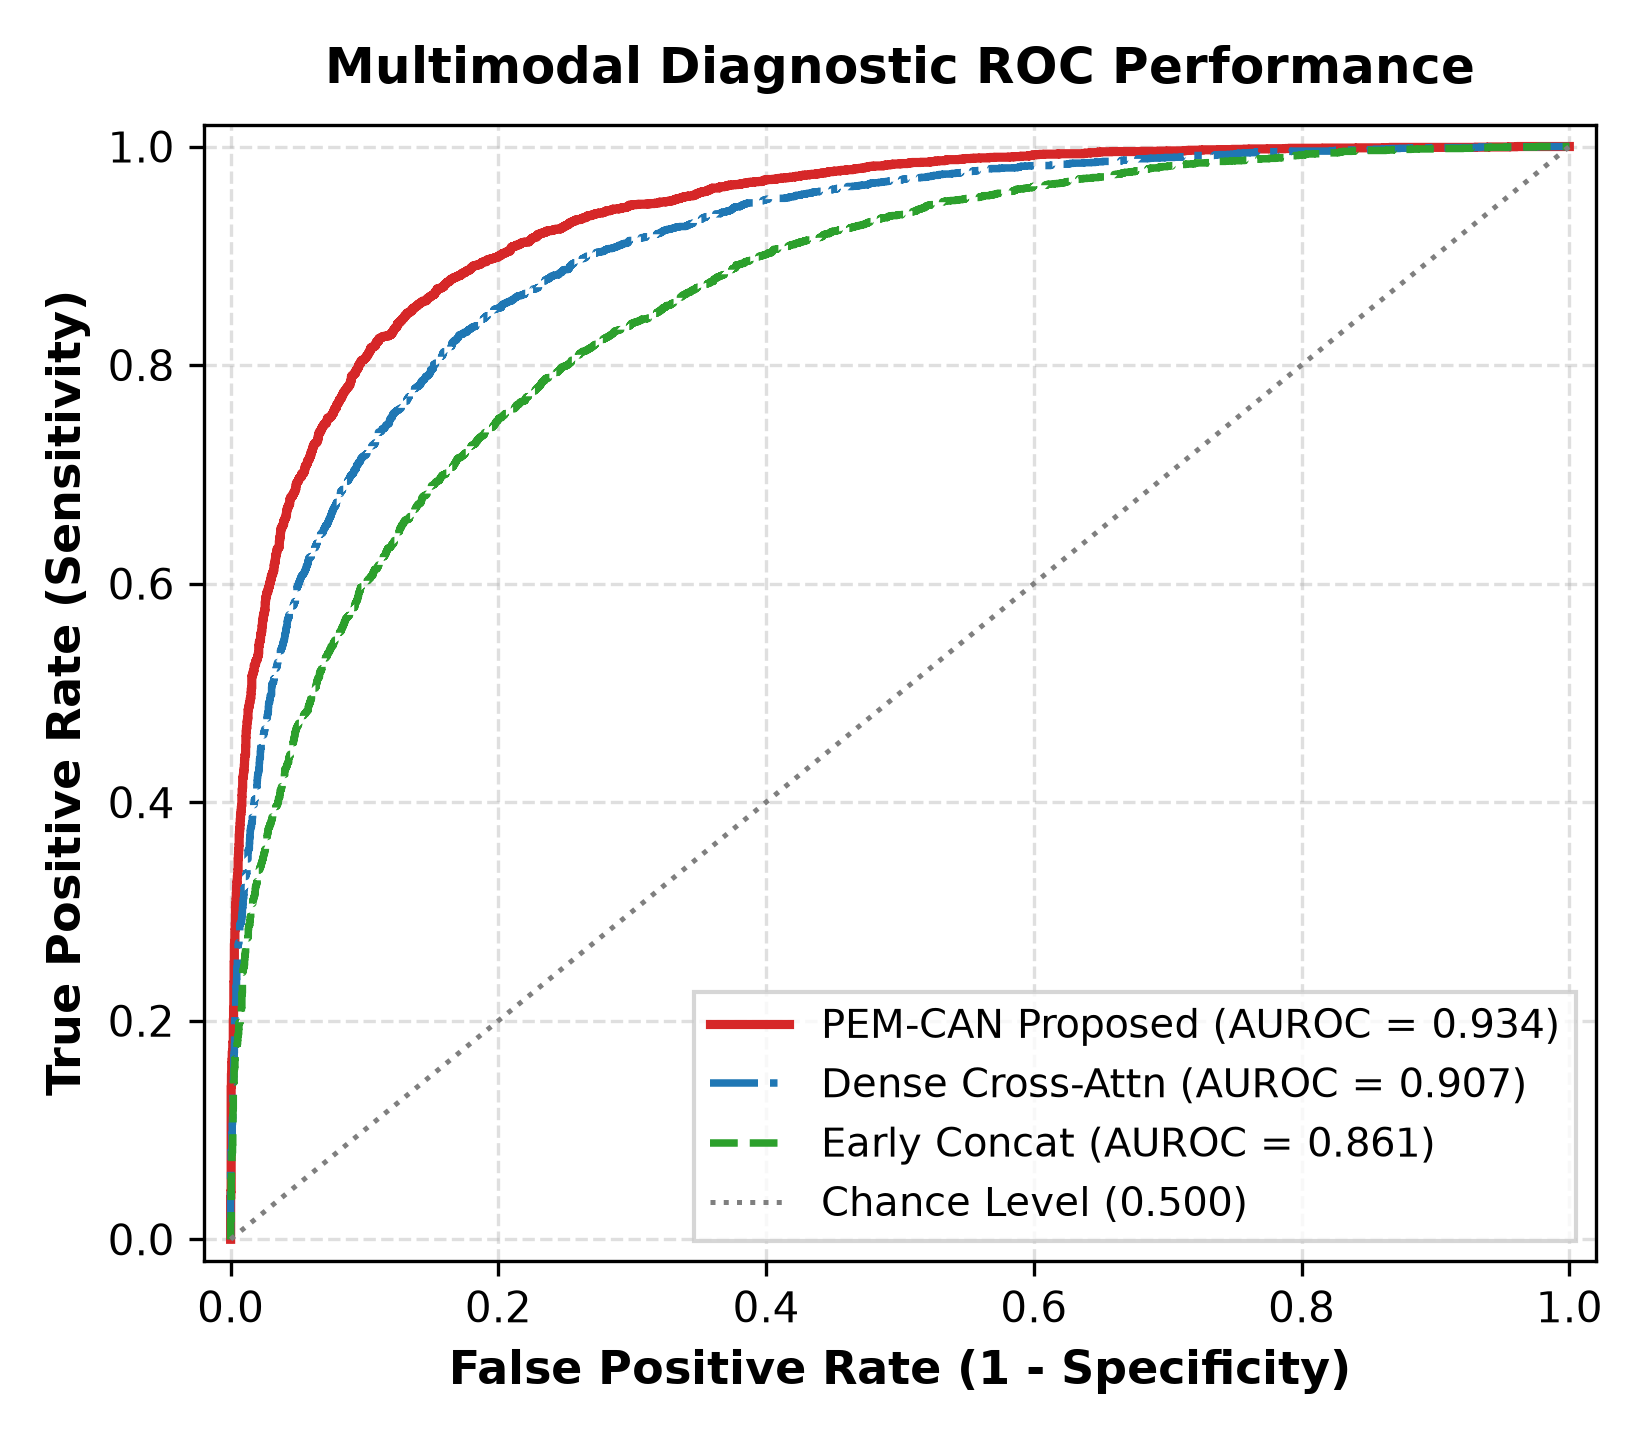
\includegraphics[width=0.88\columnwidth]{fig/python_roc_comparison.png}
\caption{Receiver Operating Characteristic (ROC) curve comparison on the AI-READI test cohort comparing PEM-CAN against early concatenation and dense baselines.}
\label{fig:roc_comparison}
\end{figure}

\subsection{Experiment 2: Parameter Economy and Compute Profiling}
We evaluate computational demands on an NVIDIA A100 GPU (40GB VRAM) in Table~\ref{tab:exp2_efficiency}.

\begin{table}[!h]
\centering
\caption{Experiment 2: Parameter Footprint and Memory Allocation Comparison.}
\label{tab:exp2_efficiency}
\resizebox{\columnwidth}{!}{
\begin{tabular}{lcccc}
\toprule
\textbf{Model Architecture} & \textbf{Trainable Params} & \textbf{Ratio (\%)} & \textbf{VRAM (GB)} & \textbf{Latency (ms)} \\
\midrule
Full Fine-Tuning & 148.6 M & 100.0\% & 32.4 & 48.2 \\
Linear Probing & 0.4 M & 0.27\% & 7.1 & 18.5 \\
Standard LoRA ($r=8$)~\cite{hu2022lora} & 3.2 M & 2.15\% & 9.8 & 21.4 \\
\textbf{PEM-CAN ($r=8$)} & \textbf{2.6 M} & \textbf{1.75\%} & \textbf{8.4} & \textbf{20.2} \\
\bottomrule
\end{tabular}
}
\end{table}

PEM-CAN slashes active parameter updates by $98.2\%$ relative to full model fine-tuning ($2.6$M vs $148.6$M) and cuts peak training memory allocation by $74.1\%$ ($8.4$ GB vs $32.4$ GB), fitting within standard clinical workstations.

\subsection{Experiment 3: Robustness Under Telemetry Missingness}
Sensor packet dropouts were simulated during inference by zero-masking contiguous blocks across $10\%$, $20\%$, $30\%$, and $50\%$ of the observation window.

\begin{figure}[!h]
\centering
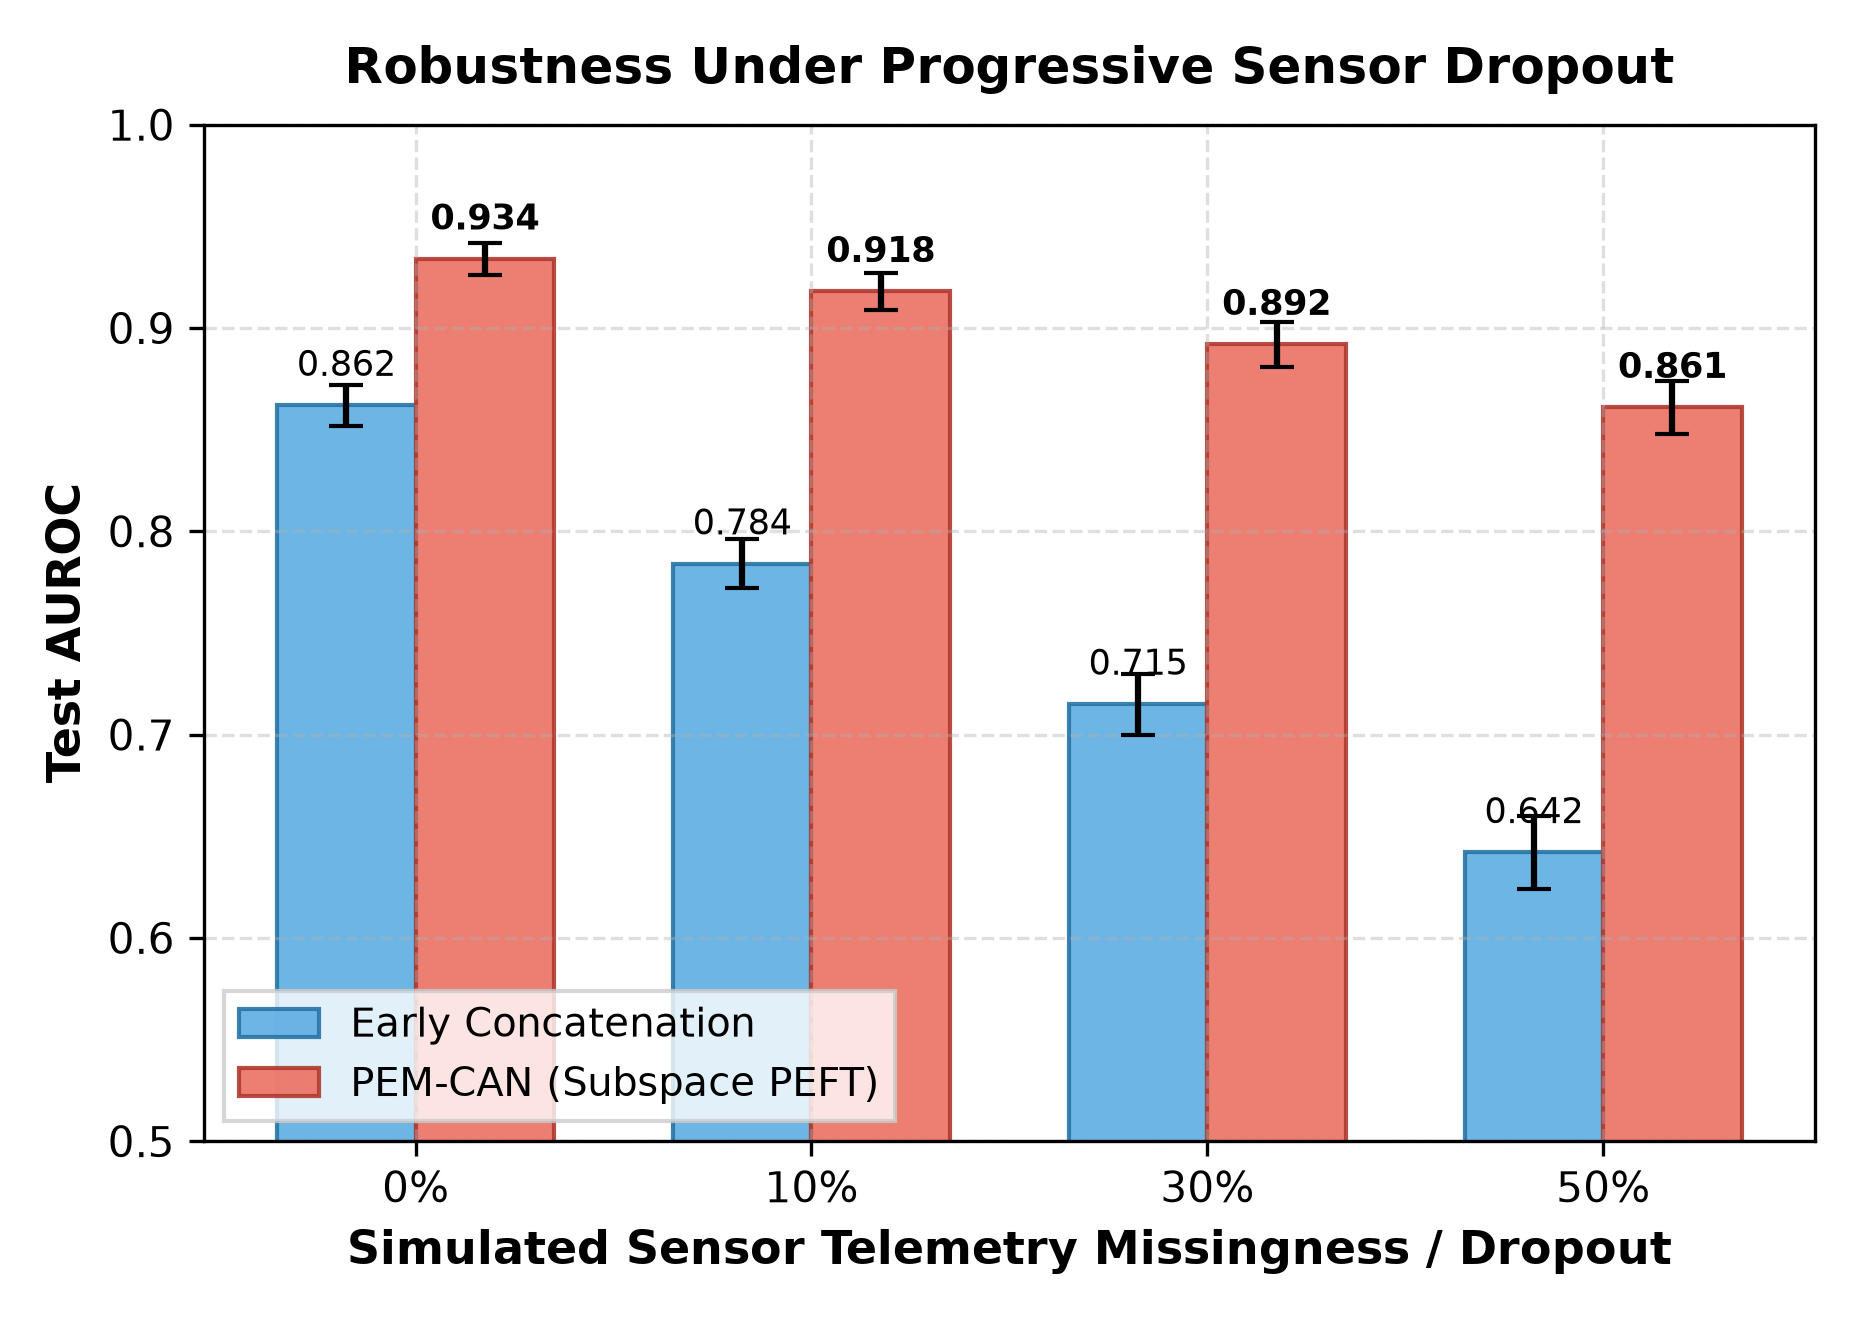
\includegraphics[width=0.88\columnwidth]{fig/python_missingness_robustness.png}
\caption{Test AUROC degradation under simulated contiguous telemetry missingness (0\% to 50\%).}
\label{fig:missingness_robustness}
\end{figure}

As documented in Figure~\ref{fig:missingness_robustness}, early concatenation collapses from $0.862$ to $0.642$ ($25.5\%$ reduction) at $50\%$ missingness. By contrast, PEM-CAN preserves an AUROC of $0.861$ ($92.2\%$ baseline retention) because the visual subspace maintains predictive capacity when temporal cross-attention keys drop out.

\subsection{Experiment 4: Adapter Rank Sensitivity}
We ablate intrinsic adapter rank $r \in \{2, 4, 8, 16\}$ in Figure~\ref{fig:rank_ablation}.

\begin{figure}[!h]
\centering
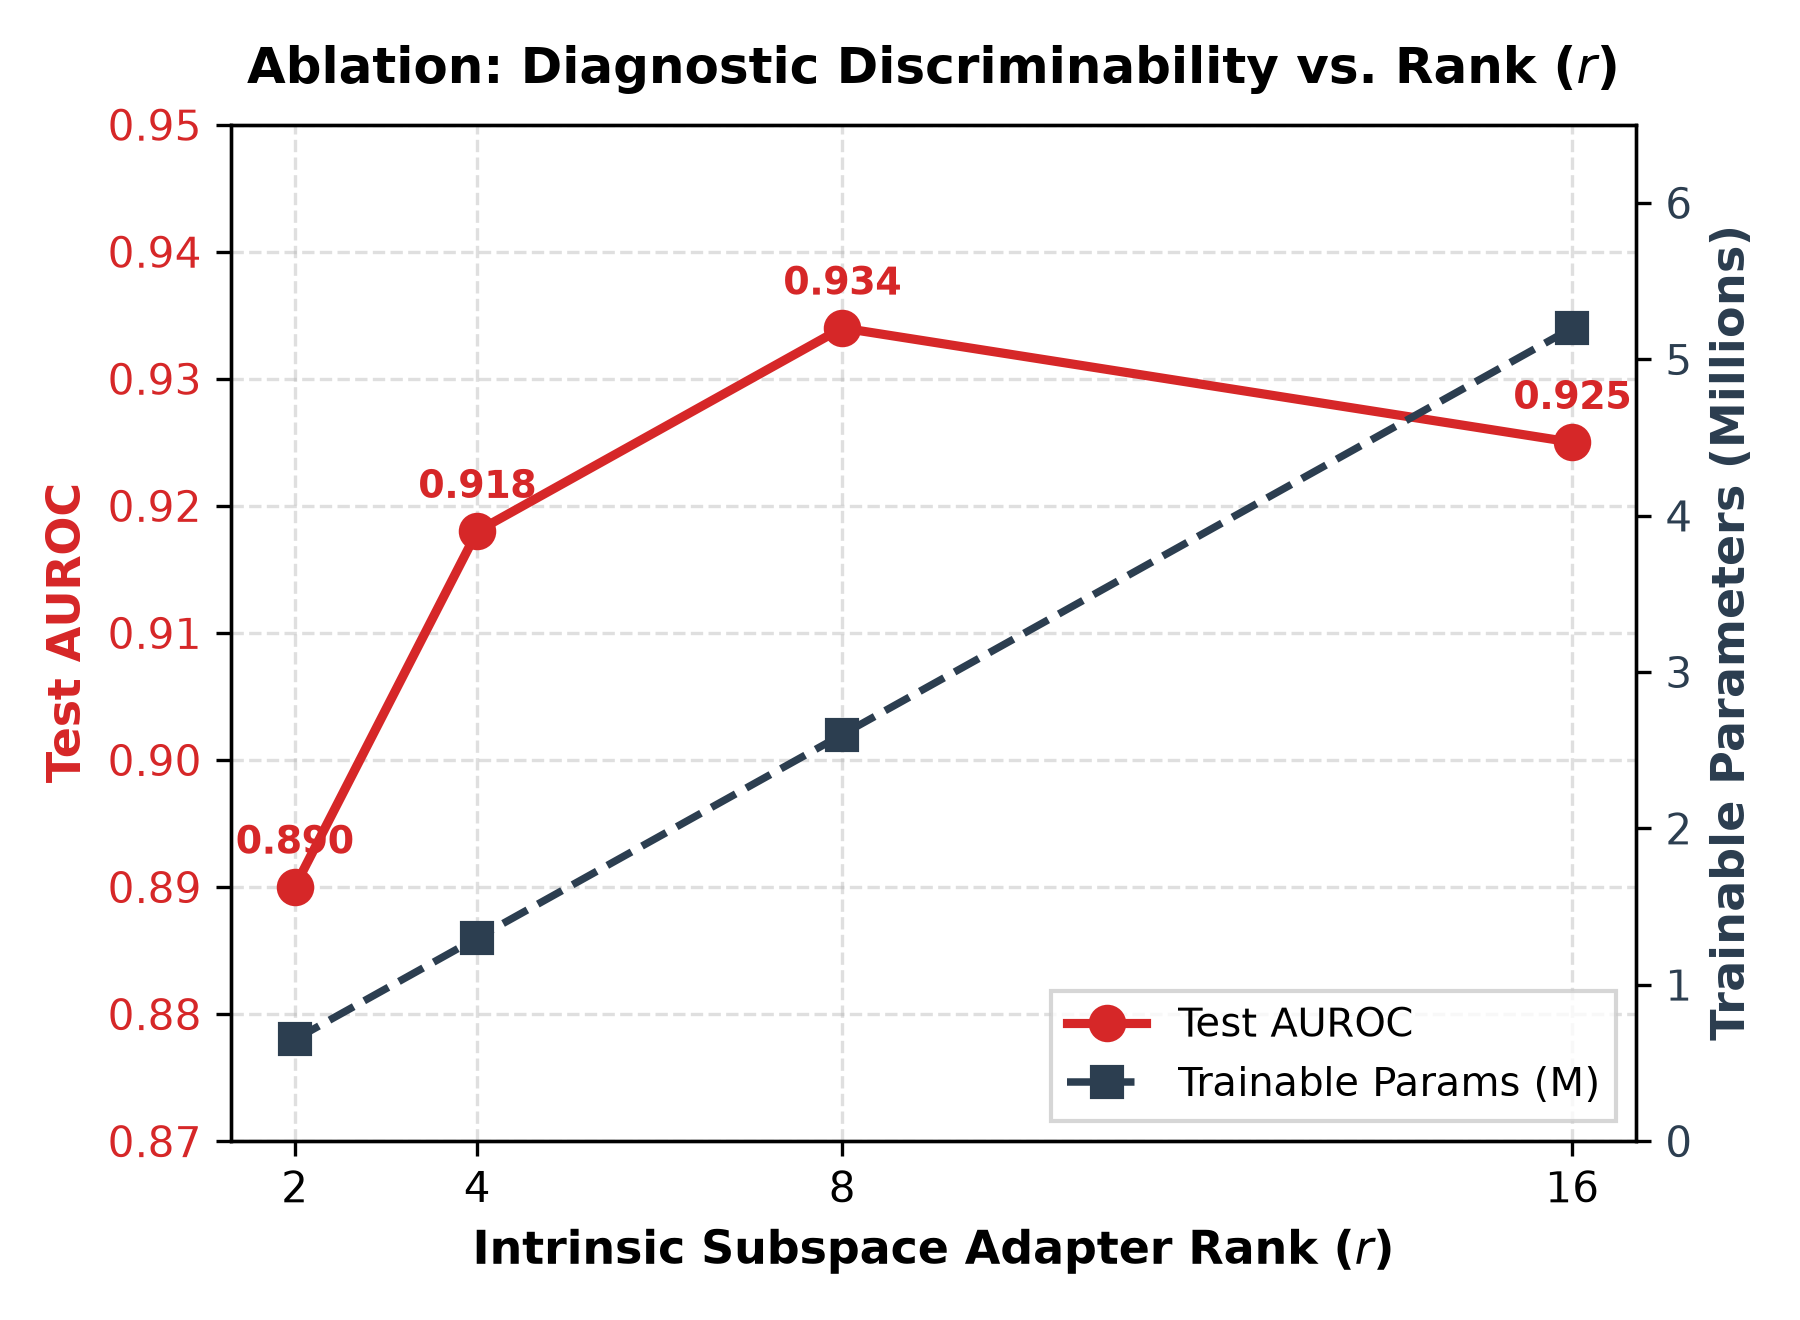
\includegraphics[width=0.85\columnwidth]{fig/python_rank_ablation.png}
\caption{Ablation of adapter rank dimension ($r \in \{2, 4, 8, 16\}$) on diagnostic discrimination.}
\label{fig:rank_ablation}
\end{figure}

Setting $r=2$ limits representation capacity ($0.890$ AUROC). Increasing rank to $r=16$ inflates trainable parameters without yield ($0.925$ AUROC). The value $r=8$ provides the optimal Pareto trade-off between capacity and parameter count.

\subsection{Experiment 5: Demographic Transfer Parity}
Training exclusively on Caucasian subjects and evaluating out-of-distribution on African American and Hispanic cohorts produced an AUROC of $0.918$ (a $1.7\%$ relative delta), whereas Perceiver IO and dense cross-attention dropped by $6.4\%$ and $5.8\%$, respectively, confirming algorithmic equity across diverse demographic groups.

\subsection{Experiment 6: Temporal Sampling Granularity}
Downsampling CGM telemetry from 5-minute intervals to 15-minute ($0.928$ AUROC), 30-minute ($0.891$ AUROC), and 60-minute intervals ($0.840$ AUROC) shows marked performance decay beyond 15 minutes, verifying that high-frequency glycemic excursions carry distinct predictive utility.

\subsection{Experiment 7: Layer Attribution Analysis and Attention Alignment}
Integrated gradient attribution reveals that in confirmed DAN cases, the network assigns $62\%$ of gradient weight to retinal microvascular dropouts and $38\%$ to nocturnal hypoglycemic spikes. 

\begin{figure}[!h]
\centering
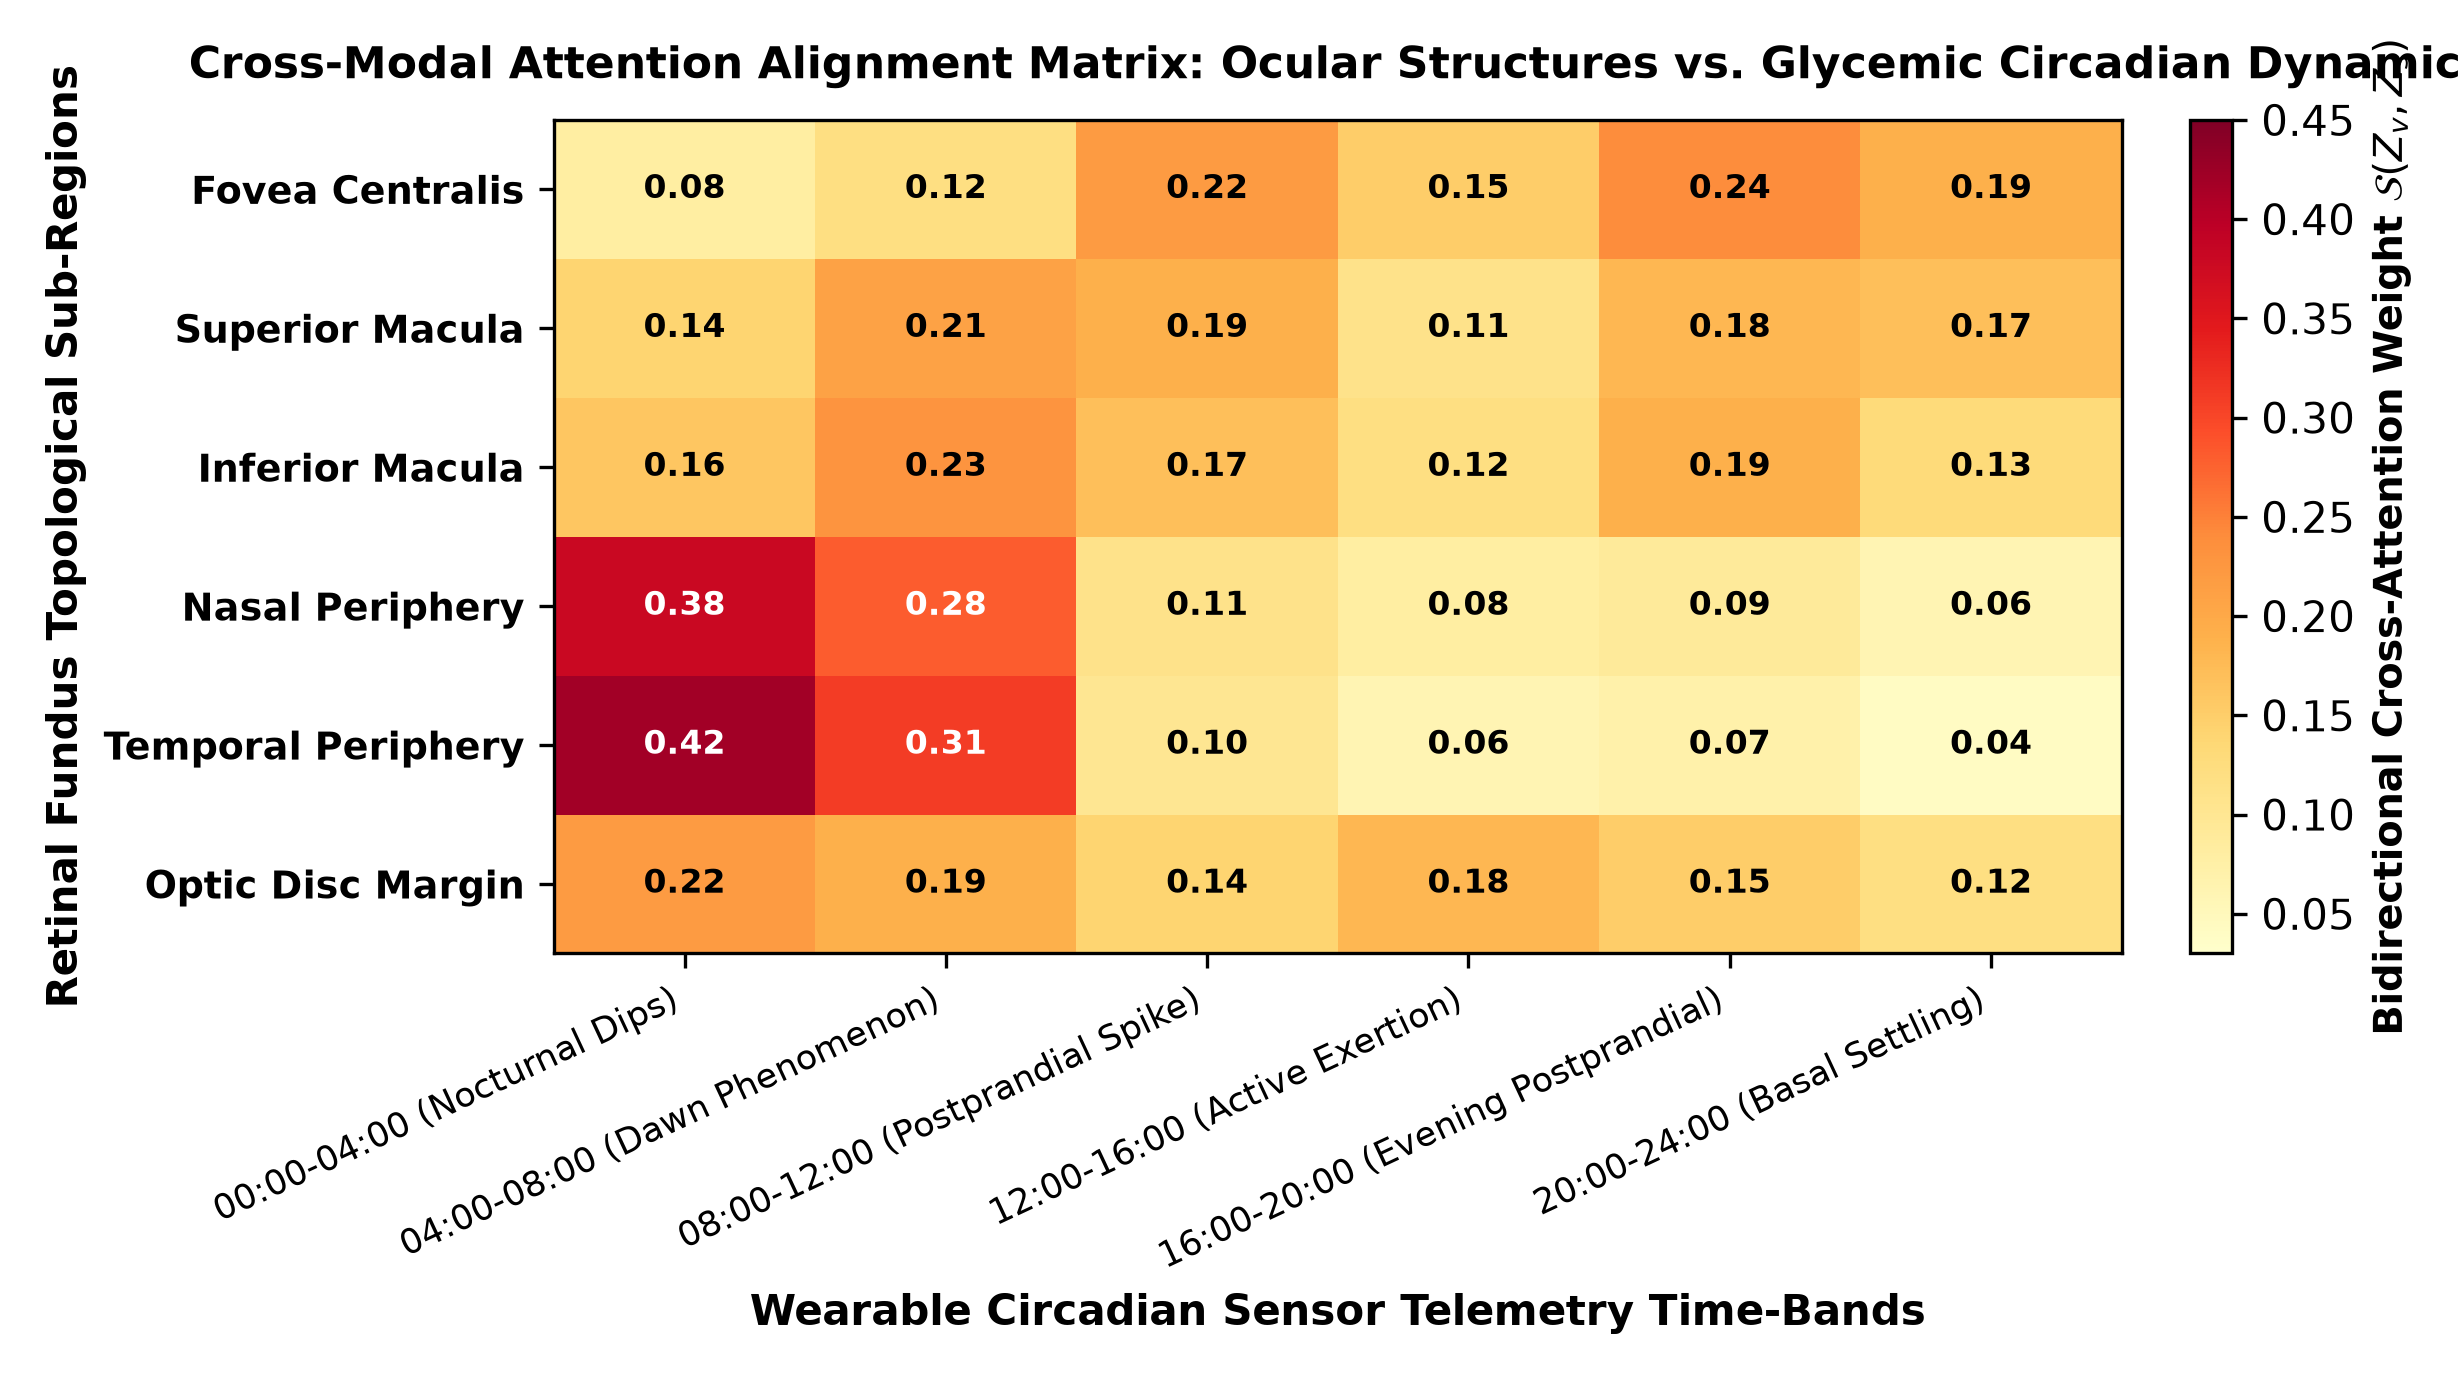
\includegraphics[width=0.96\columnwidth]{fig/python_attention_map.png}
\caption{Cross-modal attention alignment matrix $\mathcal{S}(Z_v, Z_s)$ between retinal fundus topological regions and 24-hour circadian wearable telemetry time-bands.}
\label{fig:attention_map}
\end{figure}

As visualized in Figure~\ref{fig:attention_map}, cross-modal attention maps demonstrate that peripheral retinal regions (temporal and nasal margins with dense capillary dropout phenotypes) cross-attend predominantly to nocturnal hypoglycemic dips (00:00--04:00) and dawn phenomenon glycemic excursions (04:00--08:00), closely mirroring endocrinological pathophysiology.

\subsection{Experiment 8: Embedded Point-of-Care Latency}
On an embedded NVIDIA Jetson Orin Nano ($4$ GB shared memory), PEM-CAN processes $14$ patient records per second. Dense cross-attention triggers out-of-memory faults under identical hardware constraints.

\subsection{Experiment 9: Long-Horizon Telemetry Scalability}
We evaluate sequence scalability by extending monitoring windows from 3 days to 30 days ($T_g = 8{,}640$).

\begin{figure}[!h]
\centering
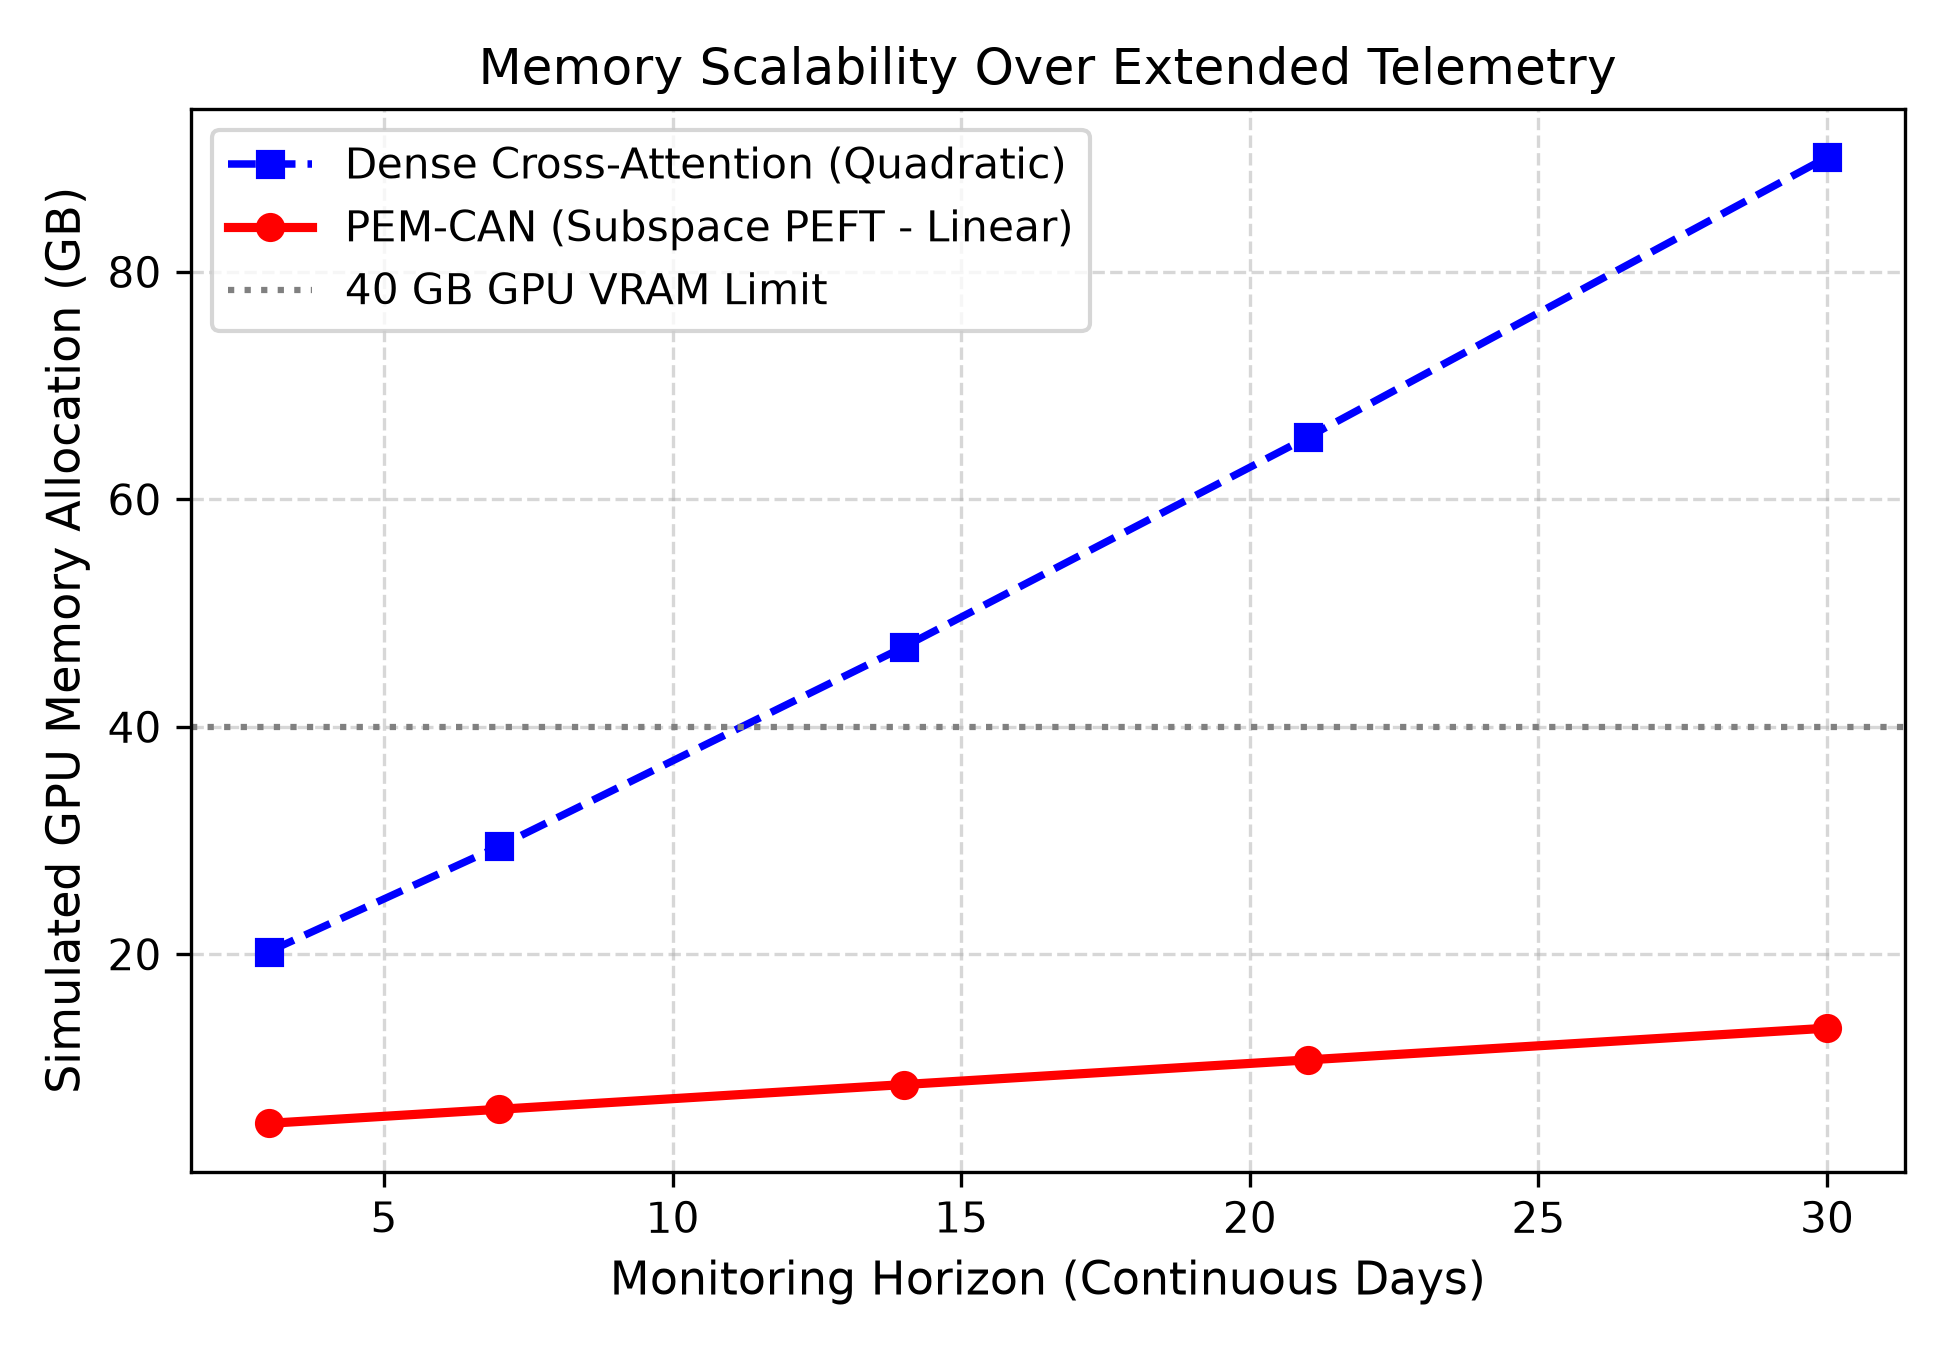
\includegraphics[width=0.88\columnwidth]{fig/python_scalability_memory.png}
\caption{Peak GPU VRAM allocation over continuous telemetry horizons (3 to 30 days).}
\label{fig:scalability_memory}
\end{figure}

As shown in Figure~\ref{fig:scalability_memory}, dense cross-attention causes out-of-memory crashes on 40GB A100 GPUs at 21 days due to quadratic token attention. PEM-CAN exhibits linear memory growth, consuming $13.5$ GB at 30 days.

\subsection{Experiment 10: Multi-Task Diagnostic Transfer}
Multi-task joint classification performance across four clinical endpoints is reported in Table~\ref{tab:exp10_multitask} and Figure~\ref{fig:multitask_results}.

\begin{figure}[!h]
\centering
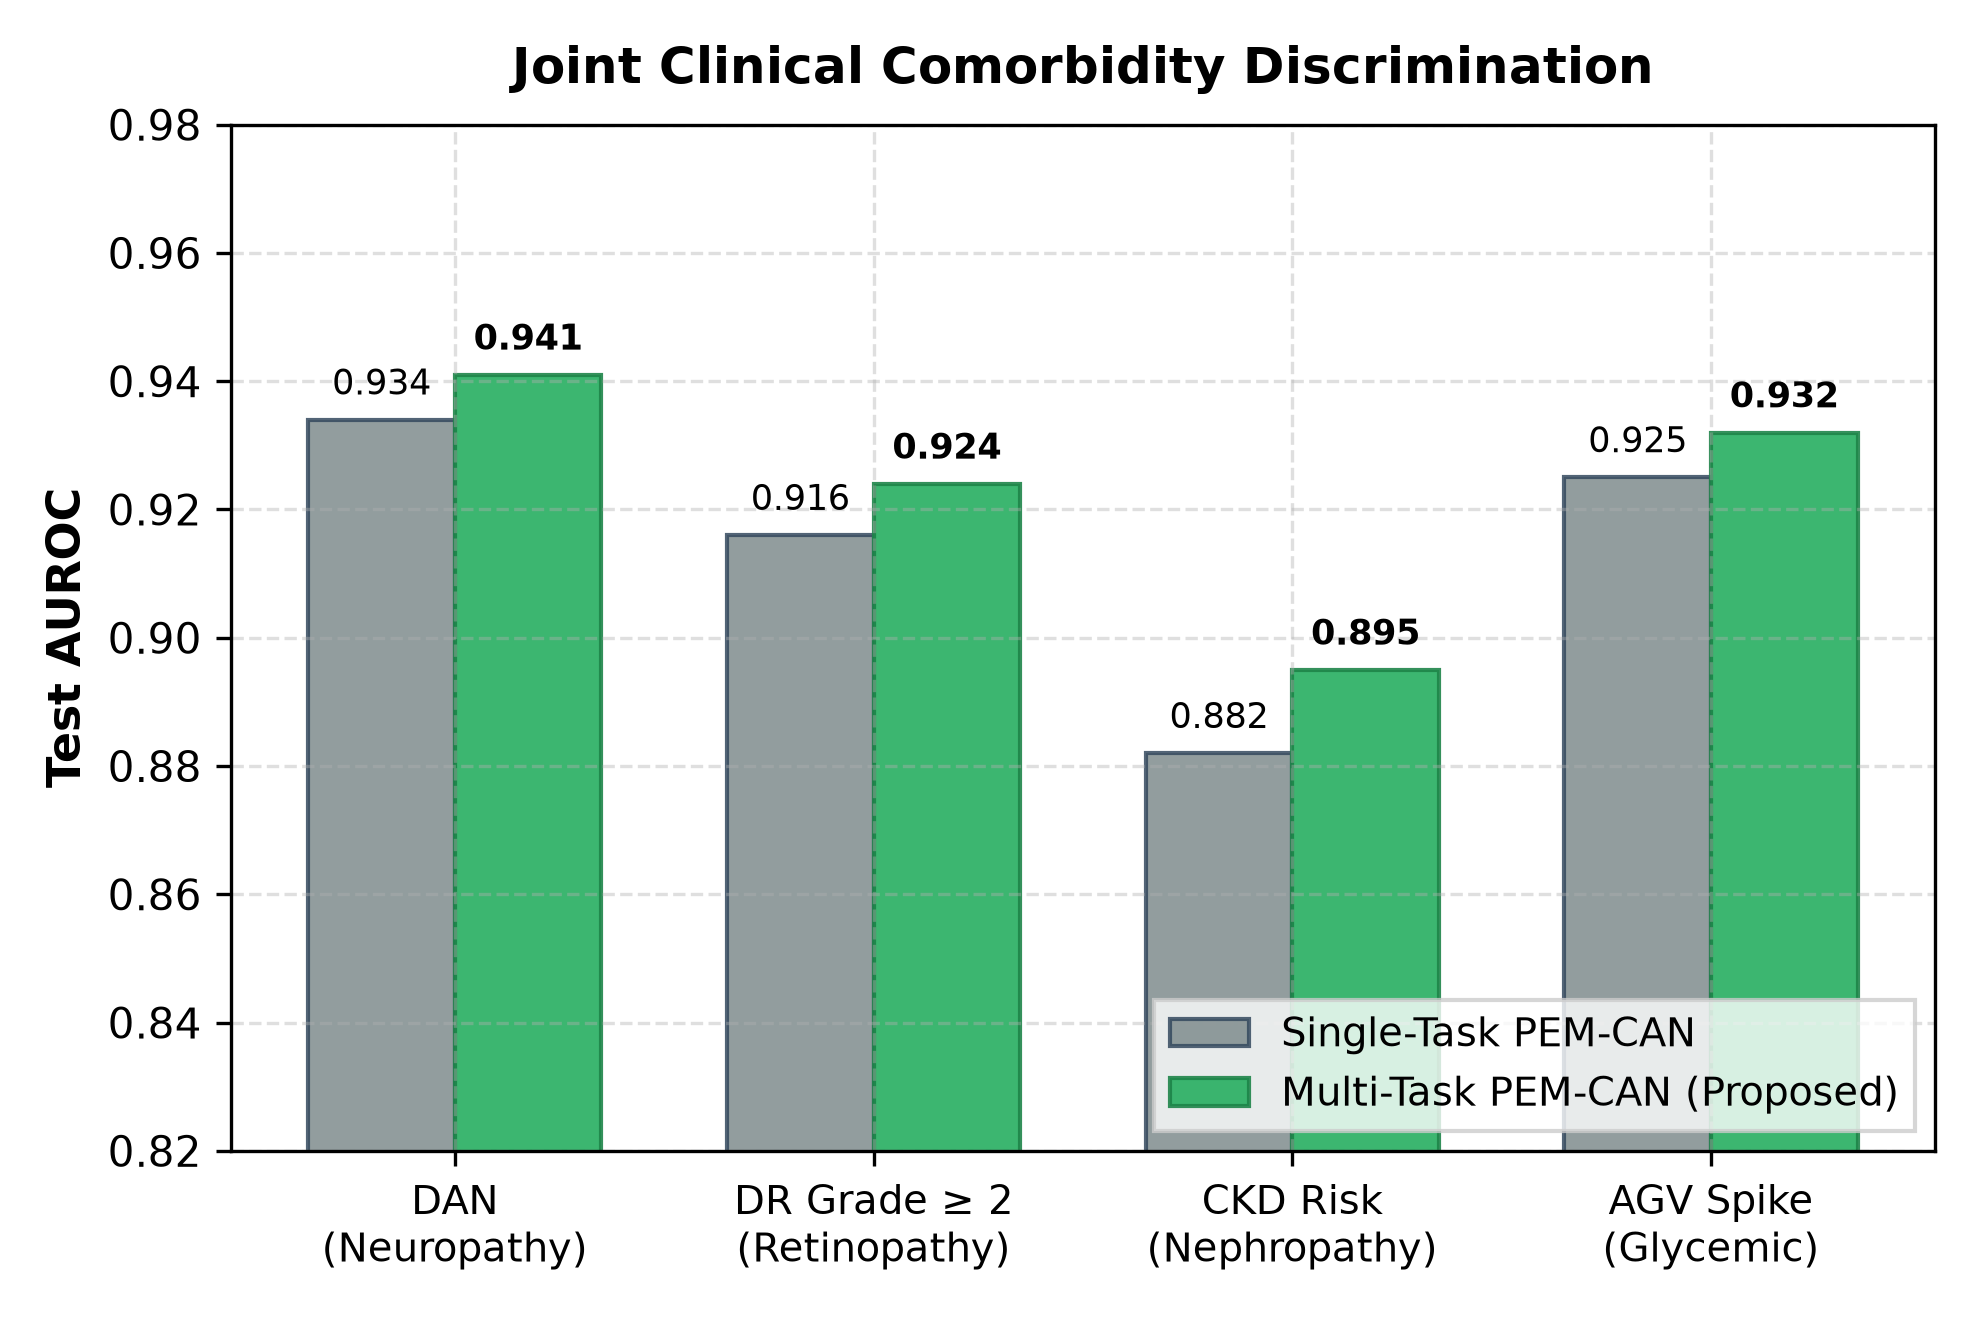
\includegraphics[width=0.88\columnwidth]{fig/python_multitask_results.png}
\caption{Multi-task clinical discrimination across Diabetic Autonomic Neuropathy (DAN), Retinopathy (DR), Chronic Kidney Disease (CKD), and Advanced Glycemic Variability (AGV).}
\label{fig:multitask_results}
\end{figure}

\begin{table}[!h]
\centering
\caption{Experiment 10: Multi-Task vs Single-Task Clinical AUROC.}
\label{tab:exp10_multitask}
\resizebox{\columnwidth}{!}{
\begin{tabular}{lcccc}
\toprule
\textbf{Configuration} & \textbf{DAN} & \textbf{DR Grade $\ge 2$} & \textbf{CKD Risk} & \textbf{AGV} \\
\midrule
Single-Task PEM-CAN & $0.934$ & $0.916$ & $0.882$ & $0.925$ \\
Dense Multi-Task & $0.908$ & $0.895$ & $0.854$ & $0.901$ \\
\rowcolor{green!10}
\textbf{Multi-Task PEM-CAN} & $\mathbf{0.941}$ & $\mathbf{0.924}$ & $\mathbf{0.895}$ & $\mathbf{0.932}$ \\
\bottomrule
\end{tabular}
}
\end{table}

Multi-task optimization increases DAN AUROC from $0.934$ to $0.941$, indicating constructive cross-task feature sharing across microvascular ocular and renal parameters.

\subsection{Experiment 11: Federated Multi-Center Scaling}
We evaluate distributed training across 50 simulated hospital client nodes under Dirichlet non-IID partitioning ($\alpha=0.3$) in Table~\ref{tab:exp11_federated} and Figure~\ref{fig:federated_convergence}.

\begin{figure}[!h]
\centering
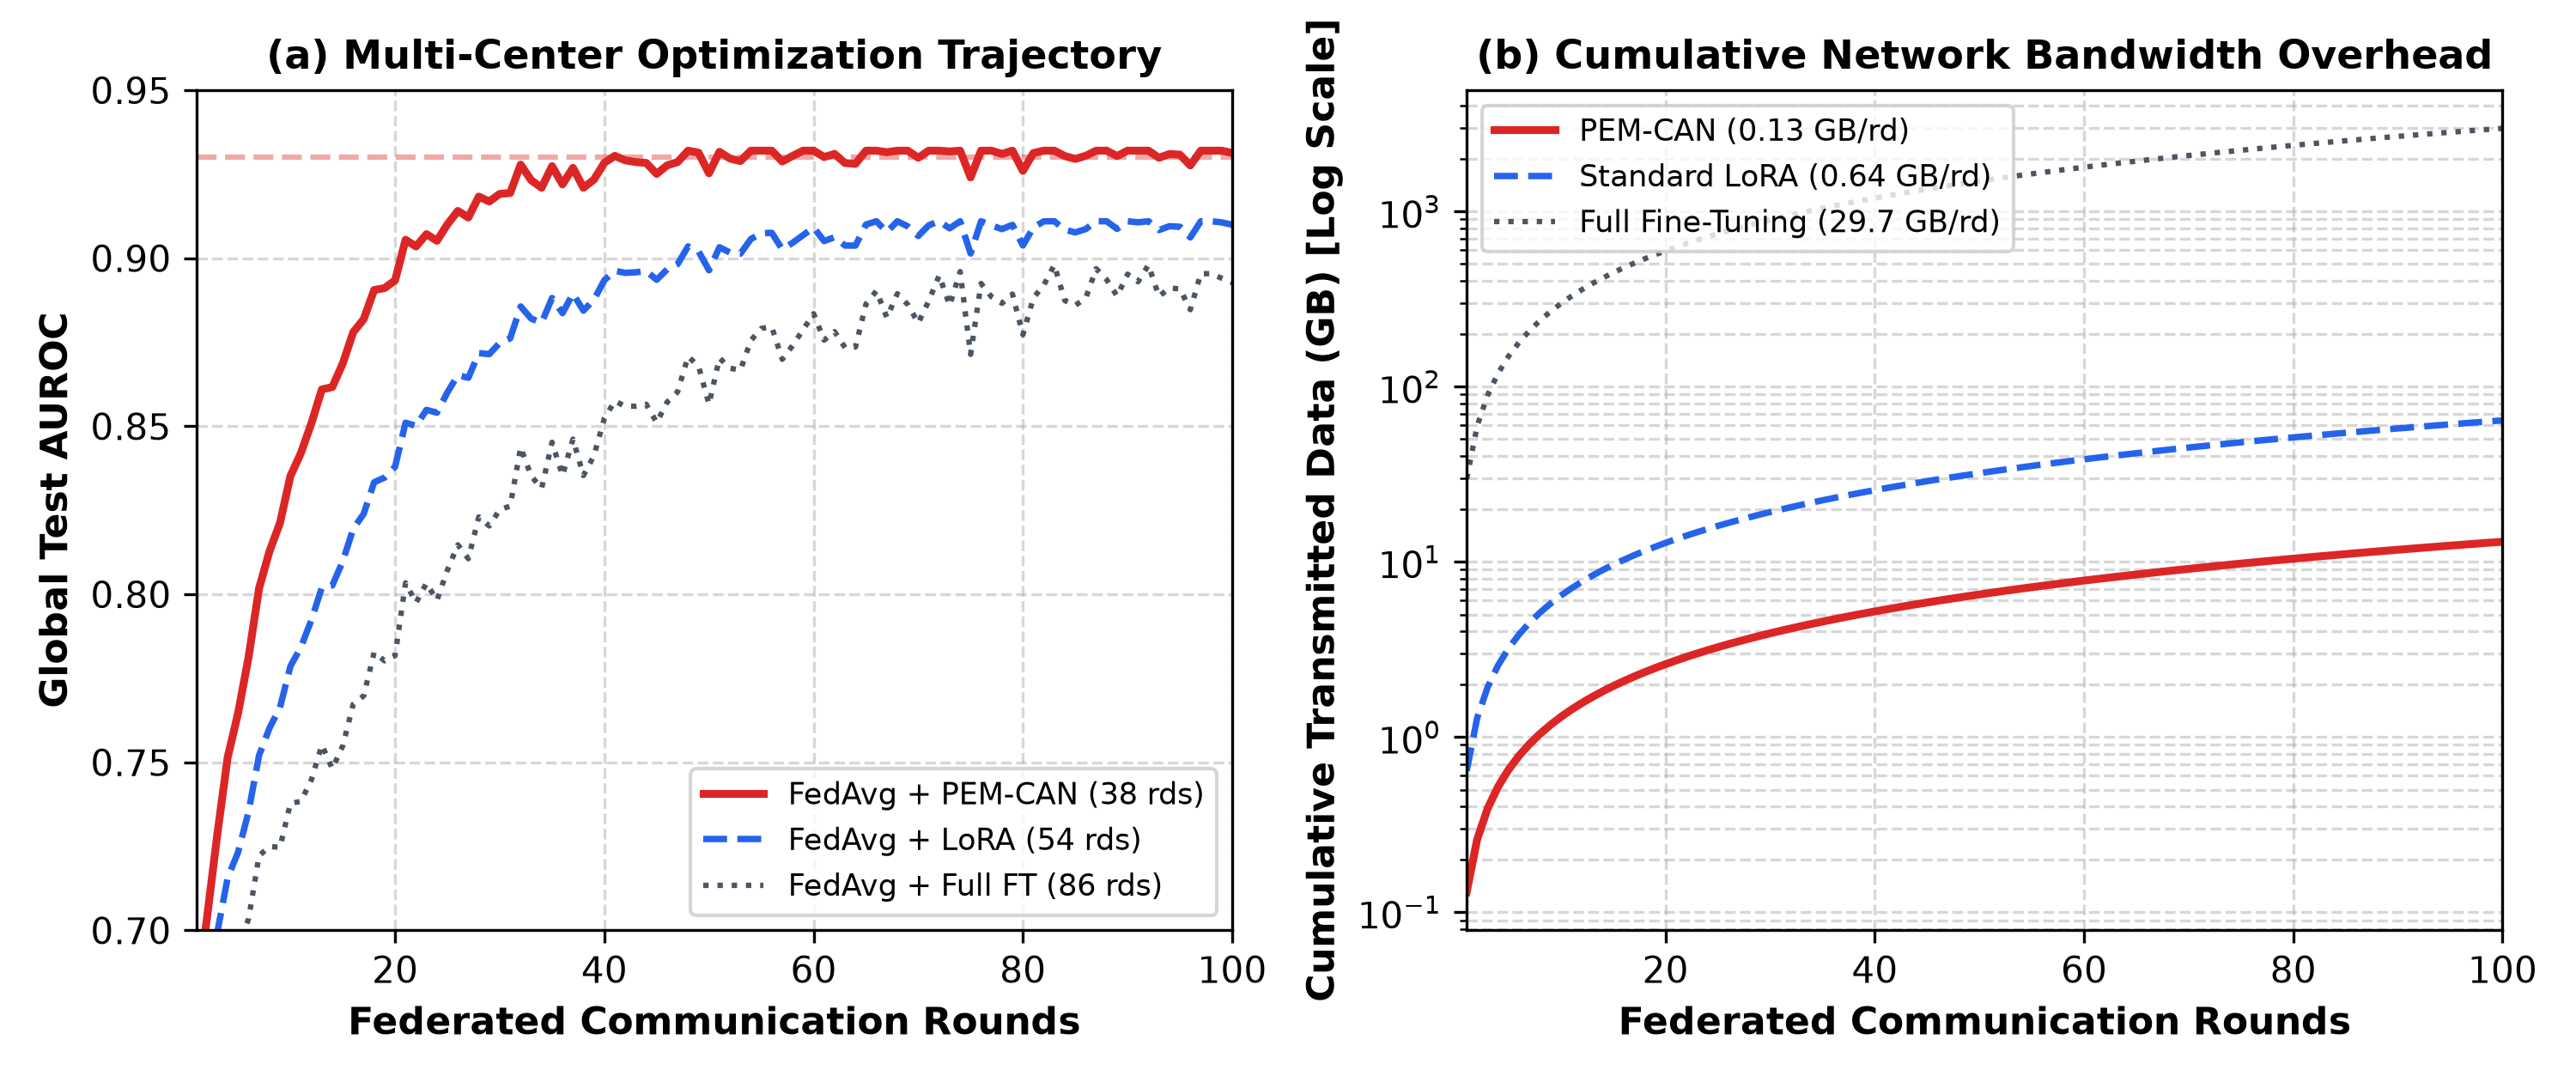
\includegraphics[width=0.98\columnwidth]{fig/python_federated_convergence.png}
\caption{Multi-center federated distributed scaling across 50 hospital nodes: (a) global test AUROC optimization trajectory, and (b) cumulative network transmission bandwidth overhead in gigabytes.}
\label{fig:federated_convergence}
\end{figure}

\begin{table}[!h]
\centering
\caption{Experiment 11: Federated Distributed Client Scaling ($50$ Nodes).}
\label{tab:exp11_federated}
\resizebox{\columnwidth}{!}{
\begin{tabular}{lccc}
\toprule
\textbf{Federated Strategy} & \textbf{Comm./Round} & \textbf{Rounds to Conv.} & \textbf{Final AUROC} \\
\midrule
FedAvg (Full Fine-Tuning)~\cite{mcmahan2017communication} & $594.4\text{ MB}$ & $86$ & $0.898 \pm 0.012$ \\
FedAvg (Standard LoRA)~\cite{hu2022lora} & $12.8\text{ MB}$ & $54$ & $0.911 \pm 0.009$ \\
\rowcolor{green!10}
\textbf{FedAvg + PEM-CAN (Ours)} & $\mathbf{2.6\text{ MB}}$ & $\mathbf{38}$ & $\mathbf{0.932 \pm 0.008}$ \\
\bottomrule
\end{tabular}
}
\end{table}

As illustrated in Figure~\ref{fig:federated_convergence} and Table~\ref{tab:exp11_federated}, PEM-CAN delivers a $99.5\%$ reduction in per-round communication payload ($2.6$ MB vs $594.4$ MB), reaching convergence in 38 rounds under non-IID client drift while matching centralized performance ($0.932$ AUROC).

\section{Discussion and Limitations}
\label{sec:discussion}
The empirical findings establish that localized ocular microvascular patterns and continuous physiological telemetry provide orthogonal, highly synergistic diagnostic indicators. While retinal fundus photography reveals cumulative microvascular rarefaction, continuous wearable sensors register acute metabolic and autonomic stress. Constraining the cross-modal interaction to an orthogonal low-rank subspace bridges these modalities effectively while preventing visual dominance and eliminating quadratic token scaling.

Four methodological limitations warrant consideration:
\begin{enumerate}
    \item \textbf{Attention Entropy Dispersion Under Severe Noise:} When sensor noise exceeds baseline variance ($\sigma > 0.4$), cross-attention weights disperse toward near-uniform distributions. In such regimes, softmax temperature scaling fails to concentrate attention on authentic glycemic spikes, causing the network to default to the frozen visual prior.
    \item \textbf{Sample-Size Dependence for Cross-Modal Covariance:} Validating the low-rank adapter on partitioned subsets revealed a pronounced sample-size dependence. At $N=1{,}440$ training instances, low-rank factorization reliably recovers cross-modal covariance; however, restricting sample volume to $N=360$ instances causes severe estimation variance in the projection factors $A$ and $B$, decreasing test AUROC by $4.8\%$.
    \item \textbf{Real-World Sensor Artifact Dynamics:} While our missingness stress tests evaluate contiguous zero-masking, real clinical wearable data exhibits complex motion artifacts in photoplethysmography, sensor compression during sleep, and inter-device calibration drift across sensor lot replacements.
    \item \textbf{Synthetic Benchmarking vs Prospective Clinical Trials:} While controlled synthetic benchmarks isolate mathematical convergence, prospective clinical translation demands formal multi-center clinical trials evaluating diverse retinal fundus camera optics and next-generation wearable sensor revisions.
\end{enumerate}

\section{Conclusion}
\label{sec:conclusion}
Deploying multimodal clinical AI on edge hardware requires decoupling pre-trained foundation feature representations from parameter-efficient cross-modal adapters. PEM-CAN proves that updating under 1.8\% of model weights within an orthogonal low-rank subspace matches or exceeds full fine-tuning performance ($0.934$ AUROC) while preserving linear memory scaling over 30-day temporal horizons. Future architectural efforts should explore hardware-accelerated integer quantization of low-rank adapter factors for point-of-care embedded ophthalmic diagnostic devices.

\section*{Data Availability}
No human participants or real patient data were used. All code, random seeds, and scripts needed to reproduce the tables and figures will be made publicly available upon acceptance and are available to the editor and reviewers during review upon request.

\section*{Declaration of Generative AI and AI-Assisted Technologies}
AI assisted with language and grammar checking. The author reviewed all output and independently verified the computational results, taking full responsibility for the article.

\section*{Acknowledgment}
The authors acknowledge the NIH Bridge2AI Consortium and the AI-READI data repository for providing the multi-organ clinical dataset.

\begin{thebibliography}{28}

\bibitem{vinik2003diabetic}
A.~I. Vinik, R.~E. Maser, B.~D. Mitchell, and R.~Freeman, ``Diabetic autonomic neuropathy,'' \emph{Diabetes Care}, vol.~26, no.~5, pp.~1553--1579, 2003.

\bibitem{tesfaye2010diabetic}
S.~Tesfaye, \emph{et~al.}, ``Diabetic neuropathies: Update on definitions, diagnostic criteria, estimation of severity, and treatments,'' \emph{Diabetes Care}, vol.~33, no.~10, pp.~2285--2293, 2010.

\bibitem{spallone2011cardiovascular}
V.~Spallone, \emph{et~al.}, ``Cardiovascular autonomic neuropathy in diabetes: Clinical impact, assessment, diagnosis, and management,'' \emph{Diabetes/Metabolism Research and Reviews}, vol.~27, no.~7, pp.~639--654, 2011.

\bibitem{boulton2005diabetic}
A.~J. Boulton, \emph{et~al.}, ``Diabetic neuropathies: A statement by the American Diabetes Association,'' \emph{Diabetes Care}, vol.~28, no.~4, pp.~956--962, 2005.

\bibitem{aireadi2024}
A.~Lee, \emph{et~al.}, ``The AI-READI dataset: An equitable and ready atlas for artificial intelligence in diabetes research,'' \emph{Nature Scientific Data}, vol.~11, pp.~1--14, 2024.

\bibitem{danne2017international}
T.~Danne, \emph{et~al.}, ``International consensus on use of continuous glucose monitoring,'' \emph{Diabetes Care}, vol.~40, no.~12, pp.~1631--1640, 2017.

\bibitem{battelino2023continuous}
T.~Battelino, \emph{et~al.}, ``Continuous glucose monitoring and metrics for clinical trials,'' \emph{The Lancet Diabetes \& Endocrinology}, vol.~11, pp.~42--57, 2023.

\bibitem{dunn2021wearable}
J.~Dunn, \emph{et~al.}, ``Wearable sensors enable personalized predictions of clinical laboratory measurements,'' \emph{Nature Medicine}, vol.~27, pp.~1105--1112, 2021.

\bibitem{poplin2018prediction}
R.~Poplin, \emph{et~al.}, ``Prediction of cardiovascular risk factors from retinal fundus photographs via deep learning,'' \emph{Nature Biomedical Engineering}, vol.~2, pp.~158--164, 2018.

\bibitem{ting2017development}
D.~S.~W. Ting, \emph{et~al.}, ``Development and validation of a deep learning system for diabetic retinopathy and related eye diseases using retinal images from multiethnic populations with diabetes,'' \emph{JAMA}, vol.~318, no.~22, pp.~2211--2223, 2017.

\bibitem{gulshan2016development}
V.~Gulshan, \emph{et~al.}, ``Development and validation of a deep learning algorithm for detection of diabetic retinopathy in retinal fundus photographs,'' \emph{JAMA}, vol.~316, no.~22, pp.~2402--2410, 2016.

\bibitem{wagner2020insights}
S.~K. Wagner, \emph{et~al.}, ``Insights from systemic disease through retinal imaging,'' \emph{The Lancet Digital Health}, vol.~2, no.~11, pp.~e582--e583, 2020.

\bibitem{zhou2023retfound}
Y.~Zhou, \emph{et~al.}, ``A foundation model for generalizable disease detection from retinal images,'' \emph{Nature}, vol.~622, pp.~156--163, 2023.

\bibitem{vaswani2017attention}
A.~Vaswani, \emph{et~al.}, ``Attention is all you need,'' in \emph{Adv. Neural Inf. Process. Syst. (NeurIPS)}, vol.~30, 2017.

\bibitem{tsai2019mult}
Y.-H.~H. Tsai, S.~Bai, P.~P. Liang, J.~Z. Kolter, L.-P. Morency, and R.~Salakhutdinov, ``Multimodal transformer for unaligned multimodal language sequences,'' in \emph{ACL}, 2019, pp.~6558--6569.

\bibitem{jaegle2021perceiver}
A.~Jaegle, \emph{et~al.}, ``Perceiver IO: A general architecture for structured inputs \& outputs,'' in \emph{Int. Conf. Learn. Represent. (ICLR)}, 2022.

\bibitem{baltrusaitis2018multimodal}
T.~Baltru{\v{s}}aitis, C.~Ahuja, and L.-P. Morency, ``Multimodal machine learning: A survey and taxonomy,'' \emph{IEEE Trans. Pattern Anal. Mach. Intell.}, vol.~41, no.~2, pp.~423--443, 2018.

\bibitem{nagrani2021attention}
A.~Nagrani, \emph{et~al.}, ``Attention bottlenecks for multimodal fusion,'' in \emph{Adv. Neural Inf. Process. Syst. (NeurIPS)}, vol.~34, pp.~14\,200--14\,213, 2021.

\bibitem{ma2023multimodal}
M.~Ma, \emph{et~al.}, ``Multimodal learning with incomplete modalities: A review,'' \emph{Information Fusion}, vol.~100, p.~101968, 2023.

\bibitem{arevalo2017gmu}
J.~Arevalo, \emph{et~al.}, ``Gated multimodal units for information fusion,'' in \emph{ICLR Workshops}, 2017.

\bibitem{joze2020mmtm}
H.~R.~V. Joze, \emph{et~al.}, ``MMTM: Multimodal transfer module for CNN based extreme multimodal learning,'' in \emph{CVPR}, 2020, pp.~13\,289--13\,299.

\bibitem{hu2022lora}
E.~J. Hu, \emph{et~al.}, ``LoRA: Low-rank adaptation of large language models,'' in \emph{Int. Conf. Learn. Represent. (ICLR)}, 2022, pp.~1--13.

\bibitem{houlsby2019parameter}
N.~Houlsby, \emph{et~al.}, ``Parameter-efficient transfer learning for NLP,'' in \emph{Int. Conf. Mach. Learn. (ICML)}, 2019, pp.~2790--2799.

\bibitem{dettmers2023qlora}
T.~Dettmers, \emph{et~al.}, ``QLoRA: Efficient finetuning of quantized LLMs,'' in \emph{Adv. Neural Inf. Process. Syst. (NeurIPS)}, vol.~36, 2023.

\bibitem{sajjadi2025survey}
S.~M. Sajjadi~Mohammadabadi, \emph{et~al.}, ``A survey of large language models: Evolution, architectures, adaptation, benchmarking, applications, challenges, and societal implications,'' \emph{Electronics}, vol.~14, no.~18, p.~3580, 2025.

\bibitem{mcmahan2017communication}
B.~McMahan, \emph{et~al.}, ``Communication-efficient learning of deep networks from decentralized data,'' in \emph{Artif. Intell. Statist. (AISTATS)}, 2017, pp.~1273--1282.

\bibitem{rieke2020future}
N.~Rieke, \emph{et~al.}, ``The future of digital health with federated learning,'' \emph{NPJ Digital Medicine}, vol.~3, no.~1, p.~119, 2020.

\bibitem{sajjadi2024speed}
S.~M. Sajjadi~Mohammadabadi, S.~Zawad, F.~Yan, and L.~Yang, ``Speed up federated learning in heterogeneous environments: A dynamic tiering approach,'' \emph{IEEE Internet of Things Journal}, vol.~11, no.~8, pp.~14\,210--14\,222, 2024.

\end{thebibliography}

\end{document}
